\documentclass{jarticle}
\usepackage{amsmath}
\usepackage{ascmac}
\usepackage{fancybox}
\usepackage[dvipdfmx]{graphicx}
\usepackage{url}
\usepackage{color}
\begin{document}
	\begin{enumerate}
		{\LARGE\item\textgt{倒立振子のモデリングと自由応答シミュレーション}}\\
		\begin{enumerate}
			{\Large\item 倒立振子のモデリング}\\
			\begin{enumerate}
				{\large\item 実験テキスト等を参考にして倒立振子の運動方程式を(台車と振り子について)求める。}\\
					
					台車の運動方程式は\\
					\begin{equation}
						M\ddot{r}=au-F_{H}-f\dot{r}
					\end{equation}
					である。\\
					倒立振子の回転の運動方程式は\\
					\begin{equation}
						J\ddot{\theta}=lF_{V}\sin \theta -lF_{H}\cos \theta -c\dot{\theta}
					\end{equation}
					である。\\
					倒立振子の水平方向の運動方程式は\\
					\begin{equation}
						m\frac{d^{2}}{dt^{2}}(r+l\sin\theta) = F_{H}
					\end{equation}
					である。\\
					倒立振子の垂直方向の運動方程式は\\
					\begin{equation}
						m\frac{d^{2}}{dt^{2}}(l\cos\theta) = F_{V}-mg
					\end{equation}
					である。\\
					
				{\large\item 導出過程を記述}\\
				
					\begin{figure}[htbp]
						\begin{center}
							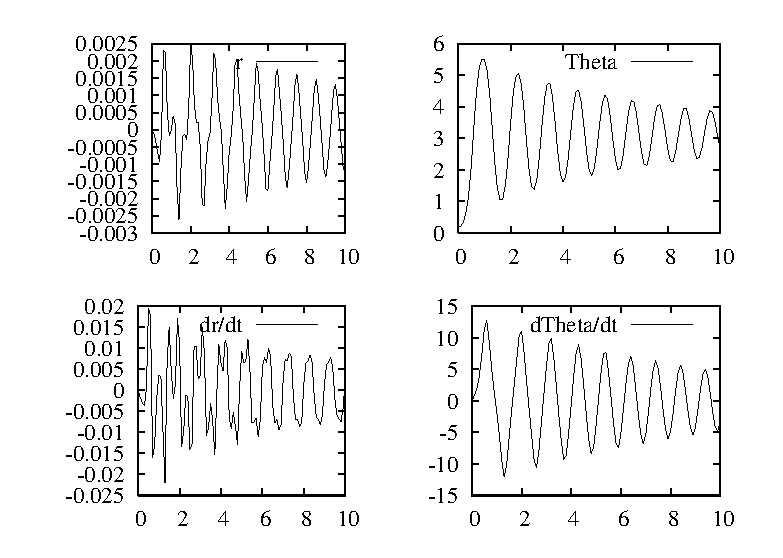
\includegraphics[width = 8cm]{gazo/InPeAboveNonLiner.eps}
						\end{center}
						\caption{台車にかかる力}
					\end{figure}
					図1より台車の運動方程式は、振り子からの水平抗力$F_{H}$を考慮してニュートンの第二法則より(1)式を導くことができる。\\
					ただし、$M$は台車の質量、$f$は台車の摩擦係数、$a$は駆動アンプへの入力電圧から台車への駆動までのゲイン、$u$はモータの駆動アンプへの入力電圧、$r$は台車の基準位置からの変位である。\\
					\\
					以下、同様にしてニュートンの第二法則を用いることで(3)、(4)式の運動方程式を導くことができる。図2を参考にするとよい\\
					\\
					\begin{figure}[htbp]
						\begin{center}
							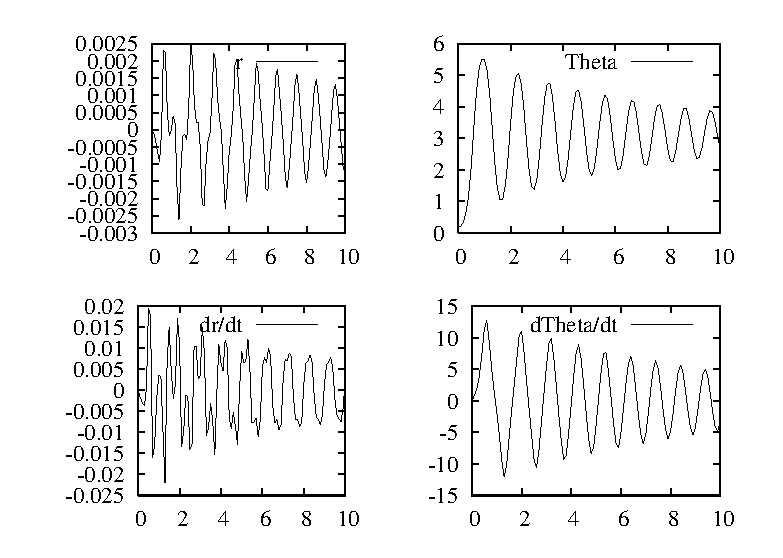
\includegraphics[width = 8cm]{gazo/InPeAboveNonLiner.eps}
						\end{center}
						\caption{振り子にかかる力}
					\end{figure}
					ただし、$m$は振り子の質量、$l$は回転軸・重心間の距離、$g$は重力加速度、$F_{V}$は振り子が台車から受ける垂直抗力である。
					また、$\theta$は鉛直上向きを$\theta=0$としたときの角度である。\\
					最後に(2)式は回転に対する運動方程式を考えることで上と同様に求めることができる。
					ただし、$J$は重心回りの慣性モーメント、$c$は回転軸摩擦係数である。\\
					
				{\large\item $x=\begin{pmatrix} r & \theta & \dot{r} & \dot{\theta} \end{pmatrix}^{\mathrm{T}}$ のように選び、(非線形モデル)非線形状態方程式$\dot{x}=f(x,u)$を導く。}\\
				
					いま、4つの状態変数から成るベクトル、すなわち状態$x$を\\
					
					\begin{eqnarray}
						x=\left[
						\begin{array}{ccc}
							r\\
							\theta\\
							\dot{r}\\
							\dot{\theta}\\
						\end{array}
						\right]
					\end{eqnarray}
					
					のように定義し、(1),(2),(3),(4)式から倒立振子系の非線形状態方程式を求める。\\
	
					\begin{eqnarray}
						\dot{x} = f(x,u) = \left[
						\begin{array}{ccc}
							\dot{r}\\
							\dot{\theta}\\
							\ddot{r}\\
							\ddot{\theta}\\
						\end{array}
						\right]
					\end{eqnarray}
					
					ここで(3)式より$F_{H}$を、(4)式より$F_{V}$を求めると\\
					
					\[F_{H} = m\frac{d^{2}}{dt^{2}}r + ml\frac{d^{2}}{dt^{2}}\sin{\theta}\]
					\begin{equation}
						    = m\ddot{r}+ml(-\dot{\theta}^{2}\sin{\theta}+\ddot{\theta}\cos{\theta})
					\end{equation}
					\\
					\[F_{V} = mg + m\frac{d^{2}}{dt^{2}}(l\cos{\theta})\]
					\begin{equation}
						= mg + ml(-\dot{\theta}^{2}\cos{\theta}-\ddot{\theta}\sin{\theta})
					\end{equation}
					\\
					(7)式を(1)式に代入すると\\
					\begin{equation}
						(M+m)\ddot{r} + ml\ddot{\theta}\cos{\theta}-ml\dot{\theta}^{2}\sin{\theta}+f\dot{r}=au
					\end{equation}
					\\
					(7)式、(8)式を(2)式に代入すると\\
					\begin{equation}
						(J + ml^{2})\ddot{\theta} + ml\ddot{r}\cos{\theta} - mgl\sin{\theta} + c\dot{\theta} = 0
					\end{equation}
					\\
					(9)式、(10)式を行列表現すると\\
					\begin{eqnarray}
						\left[
						\begin{array}{ccc}
							(M + m)\ddot{r} + (ml\cos{\theta})\ddot{\theta} + (-ml\sin{\theta}) + f\dot{r} = au \\
							(ml\cos{\theta})\ddot{r} + (J + ml^{2})\ddot{\theta} -mgl\sin{\theta} + c\dot{\theta} = 0\\
						\end{array}
						\right]
					\end{eqnarray}
					\begin{eqnarray}
						\left[
						\begin{array}{ccc}
							M + m & ml\cos{\theta} \\
							ml\cos{\theta} & J + ml^{2}\\
						\end{array}
						\right]
						\left[
						\begin{array}{ccc}
							\ddot{r} \\
							\ddot{\theta}\\
						\end{array}
						\right] +
						\left[
						\begin{array}{ccc}
							-ml\ddot{\theta}^{2}\sin{\theta} + f\dot{r}\\
							mgl\sin{\theta} + c\dot{\theta}\\
						\end{array}
						\right] = 
						\left[
						\begin{array}{ccc}
							au\\
							0\\
						\end{array}
						\right]
					\end{eqnarray}
					\\
					$\begin{pmatrix} M + m & ml\cos{\theta} \\ ml\cos{\theta} & J + ml^{2} \end{pmatrix}$を$K$と置いて右辺に逆行列としてかけると\\
					\begin{equation}
						\left[
						\begin{array}{ccc}
							\ddot{r}\\
							\ddot{\theta}\\
						\end{array}
						\right]=K^{-1}
						\left[
						\begin{array}{ccc}
							au-f\dot{r}+ml\ddot{\theta}\sin{\theta}\\
							mgl\sin{\theta} - c\dot{\theta}\\
						\end{array}
						\right]
					\end{equation}
					\\
					よって以上から(6)式は\\
					\begin{equation}
						\dot{x} = f(x,u)=\left[
						\begin{array}{ccc}
							\dot{r}\\
							\dot{\theta}\\
							K^{-1}\left[
							\begin{array}{ccc}
								-f\dot{r}+ml\ddot{\theta}\sin{\theta}+au\\
								mgl\sin{\theta}-c\dot{\theta}
							\end{array}
							\right]
						\end{array}
						\right]
					\end{equation}
					\\
					となる。ただし、$K$は
					\begin{equation}
					K=\left[
					\begin{array}{ccc}
						M+m & ml\cos{\theta}\\
						ml\cos{\theta} & J+ml^{2}\\
					\end{array}
					\right]
					\end{equation}
					\\
					である。
					\\
	
				{\large\item 平衡点$x=\begin{pmatrix} 0 & 0 & 0 & 0 \end{pmatrix}^{\mathrm{T}}$近傍で線形化し、(線形モデル)線形状態方程式$\dot{x}=Ax+Bu$と出力方程式$y=Cx$を導く。}\\	
				
					この時、この基準状態まわりで(15)式を一次近似することを考える。\\
					(15)式に一次近似のテイラー展開を施すと、\\
					\begin{equation}
						f(x,u) = f(0,0) + \left.\frac{\partial f}{\partial x}\right|_{x=0,u=0}(x-0) + \left.\frac{\partial f}{\partial u}\right|_{x=0,u=0}(u-0)
					\end{equation}
					\\
					となる。\\
					また、$A=\left.\frac{\partial f}{\partial x}\right|_{x=0,u=0} , B=\left.\frac{\partial f}{\partial u}\right|_{x=0,u=0}$とする。\\
					ここで、一時近似を施したので、$\theta$を微小範囲と考えることができ、$\sin{\theta} \simeq  \theta , \cos{\theta} \simeq 1 , \dot{\theta}^{2} \simeq 0$のように
					近似できる。\\
					以上の近似を(14)、(15)式に適用すると\\
					\begin{equation}
						f(x,u)=\left[
						\begin{array}{ccc}
							\dot{r}\\
							\dot{\theta}\\
							K^{'-1}\left[
							\begin{array}{ccc}
								au-f\dot{r}\\
								mlg\theta-c\dot{\theta}\\
							\end{array}
							\right]
						\end{array}
						\right]
					\end{equation}
					\begin{equation}
						K^{'} = \left[
						\begin{array}{ccc}
							M + m & ml\\
							ml & J+ml^{2}\\
						\end{array}
						\right]
					\end{equation}
					\\
					(17)、(18)式を用いてA、Bを計算する\\
					ここで、(17)式の3行目を$a_{1}$と置き、4行目を$a_{2}$と置く。\\
					\begin{equation}
						A=\frac{\partial \textgt{f}}{\partial \textgt{x}}=\\
						\left[
						\begin{array}{cccc}
							\frac{\partial \dot{r}}{\partial r} & \frac{\partial \dot{r}}{\partial \theta} & \frac{\partial \dot{r}}{\partial \dot{r}} & \frac{\partial \dot{r}}{\partial \dot{\theta}} \\
							\frac{\partial \dot{\theta}}{\partial r} & \frac{\partial \dot{\theta}}{\partial \theta} & \frac{\partial \dot{\theta}}{\partial \dot{r}} & \frac{\partial \dot{\theta}}{\partial \dot{\theta}} \\
							\frac{\partial a_{1}}{\partial r} & \frac{\partial a_{1}}{\partial \theta} & \frac{\partial a_{1}}{\partial \dot{r}} & \frac{\partial a_{1}}{\partial \dot{\theta}} \\
							\frac{\partial a_{2}}{\partial r} & \frac{\partial a_{2}}{\partial \theta} & \frac{\partial a_{2}}{\partial \dot{r}} & \frac{\partial a_{2}}{\partial \dot{\theta}} \\
						\end{array}
						\right]\\
					\end{equation}
					\begin{equation}
						=\left[
						\begin{array}{cccc}
							0 & 0 & 1 & 0 \\
							0 & 0 & 0 & 1 \\
							0 & 0 & K^{'-1}(-f) & 0\\
							0 & K^{'-1}(mgl) & 0 & K^{'-1}(-c) \\
						\end{array}
						\right]
					\end{equation}
					\\
					\begin{equation}
						B=\frac{\partial \textgt{f}}{\partial \textgt{u}}=
						\left[
						\begin{array}{c}
							\frac{\partial \dot{r}}{\partial u}\\
							\frac{\partial \dot{\theta}}{\partial u}\\
							\frac{\partial a_{1}}{\partial u}\\
							\frac{\partial a_{2}}{\partial u}\\
						\end{array}
						\right]=
						\left[
						\begin{array}{c}
							0\\
							0\\
							K^{'-1}a\\
							0\\
						\end{array}
						\right]
					\end{equation}
					\\
					よって線形状態方程式は\\
					\[\dot{x}=A\textgt{x}+B\textgt{u}\]
					\begin{equation}
						=\left[
						\begin{array}{cccc}
							0 & 0 & 1 & 0 \\
							0 & 0 & 0 & 1 \\
							0 & 0 & K^{'-1}(-f) & 0 \\
							0 & K^{'-1}(mgl) & 0 & K^{'-1}(-c)\\
						\end{array}
						\right]
						\left[
						\begin{array}{c}
							r\\
							\theta\\
							\dot{r}\\
							\dot{\theta}\\
						\end{array}
						\right] + 
						\left[
						\begin{array}{c}
							0\\
							0\\
							K^{'-1}au\\
							0\\
						\end{array}
						\right]
					\end{equation}
					\\
					また、出力方程式は2つの観測出力は
					\begin{equation}
						y_{1} = c_{1}r\\
					\end{equation}
					\begin{equation}
						y_{2} = c_{2}\theta\\
					\end{equation}
					のように表される。ここで、$c_{1}$は変位・電圧変換係数、$c_{2}$は角度・電圧変換係数である。これから成るベクトル出
					力$y$を\\
					\begin{equation}
						y=\left[
						\begin{array}{c}
							y_{1}\\
							y_{2}\\
						\end{array}
						\right]
					\end{equation}
					のように定義すると、倒立振子系に対する観測方程式として\\
					\begin{equation}
						y=Cx
					\end{equation}
					\begin{equation}
						\left[
						\begin{array}{c}
							y_{1}\\
							y_{2}\\
						\end{array}
						\right]=\left[
						\begin{array}{cccc}
							c_{1} & 0 & 0 & 0 \\
							0 & c_{2} & 0 & 0\\
						\end{array}
						\right]\left[
						\begin{array}{c}
							r\\
							\theta\\
							\dot{r}\\
							\dot{\theta}\\
						\end{array}
						\right]
					\end{equation}
					を得ることができる。\\
					
				
			\end{enumerate}
			{\Large\item 非線形モデルに基づく自由応答シミュレーション}\\
			\begin{enumerate}
				{\large\item 倒立振子の非線形モデルの状態の微分(ベクトル)
	 		   	$\dot{x}=\begin{bmatrix} \dot{r} & \dot{\theta} & \ddot{r} & \ddot{\theta} \end{bmatrix}^{\mathrm{T}}$
	 		   	を返す関数\textgt{diff\_eqs()}を書く。}\\
	 		   	
	 		   		以下に、MaTXで作成したdiff\_eqs()を以下に示す。\\
	 		   		\begin{itembox}[l]{diff\_eqs()}
	 		   			// diff\_eqs() は微分方程式を記述する関数\\
						Func void diff\_eqs(DX,t,X,UY)\\
						// tは時間\\
						Real t;\\
						Matrix X,DX,UY;\\
						\{\\
							Real M,m,l,J,f,a,c,g,r,th,dr,dth;\\
							Real xp2size;\\
							Matrix xp,up,dxp;\\
							Matrix K,KZ,CO,SI;\\
							Integer i;\\
							\\
							//物理パラメータの設定\\
							M=1.49;        m=0.038; l=0.13;\\
							J=4.5E-4; f=15.10; a=0.73;\\
							c=2.1E-4; g=9.8;\\
							\\
							//Xはx=(r Theta dr/dt dTheta/dt)\^Tを表す\\
							xp = X;\\
							// Uyは入力\\
							up = UY;\\
							\\
							r=X(1,1);\\
							th=X(2,1);\\
							dr=X(3,1);\\
							dth=X(4,1);\\
							\\
							K=[[M + m           , m * l * cos(th)  ]
							     [m * l * cos(th) , J + m * l * l    ]];
							\\
							KZ=[[    -f*dr      + m*l*sin(th)*dth*dth + a * up(1,1)]
								[ m*g*l*sin(th) - c*dth            ]];\\
							\\
							dxp=[[X(3:4,1)][K\textbackslash KZ]];\\
							DX \ = [dxp];\\
						\}\\
					\end{itembox}
					\\
	 		   	
				{\large\item 入力を0とし、真上から$(0^\circ~20^\circ)$傾けたところから離した場合のシミュレーションを実行する。シミュ
				レーションには関数Odeを用いる}\\
				
					以下にシミュレーションを行った出力結果を示す。\\
					左から$r , \theta , \dot{r} , \dot{\theta}$である。ただし、シミュレーションは10秒間行う。データ行が101個あるので、最
					初の0秒目のデータと最後の10秒目のデータを以下に示す。
					\begin{itembox}[l]{XC(出力結果)}
						\# 4 101\\
						0.00000000E+000  1.74532925E-001  0.00000000E+000  0.00000000E+000\\
						省略\\
						-1.20435914E-003  2.64681608E+000  2.46294987E-003 -3.33770438E+000\\
					\end{itembox}
				
				{\large\item 得られたデータをプロットする(mgplot利用)}\\
				
					以下にmgplotを用いてデータをプロットした結果を示す。\\
					\begin{figure}[htbp]
						\begin{center}
							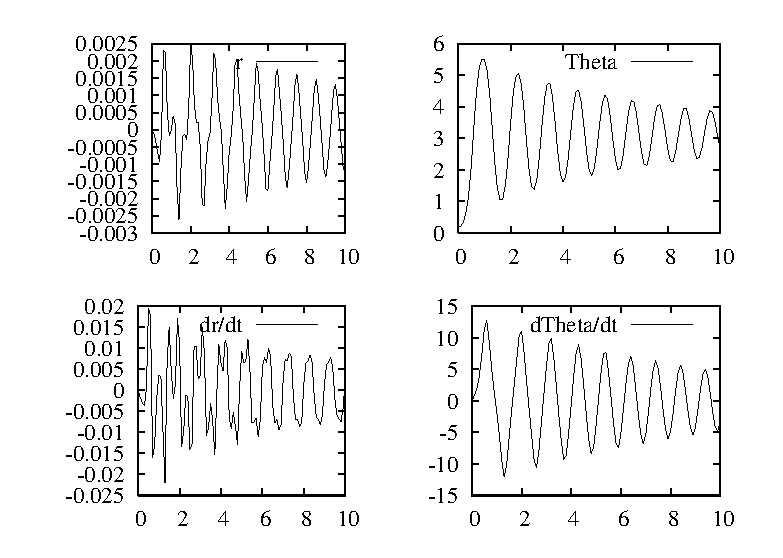
\includegraphics[width=8cm]{gazo/InPeAboveNonLiner.eps}\\
						\end{center}
						\caption{データのプロット結果}
					\end{figure}
					\\
				
				{\large\item グラフをEPSファイルに保存する。}\\
				
					上の図3はグラフをepsファイルに保存したものを貼り付けている。epsファイルを生成するために使用するコマンドはmgplot
					$\_$eps(1,''data.eps'')でファイルに保存することができる。\\
				
				{\large\item EPSファイルをPDFファイルに変換する}\\
				
					以下のウェブサイトにアクセスすることでEPSファイルをPDFファイルに変換することができる。\\
					\textcolor{cyan}{\url{https://convertio.co/ja/vector-converter/}}\\
					\\
					以下に変換したpdfファイルを示す。\\
					\begin{figure}[htbp]
						\begin{center}
							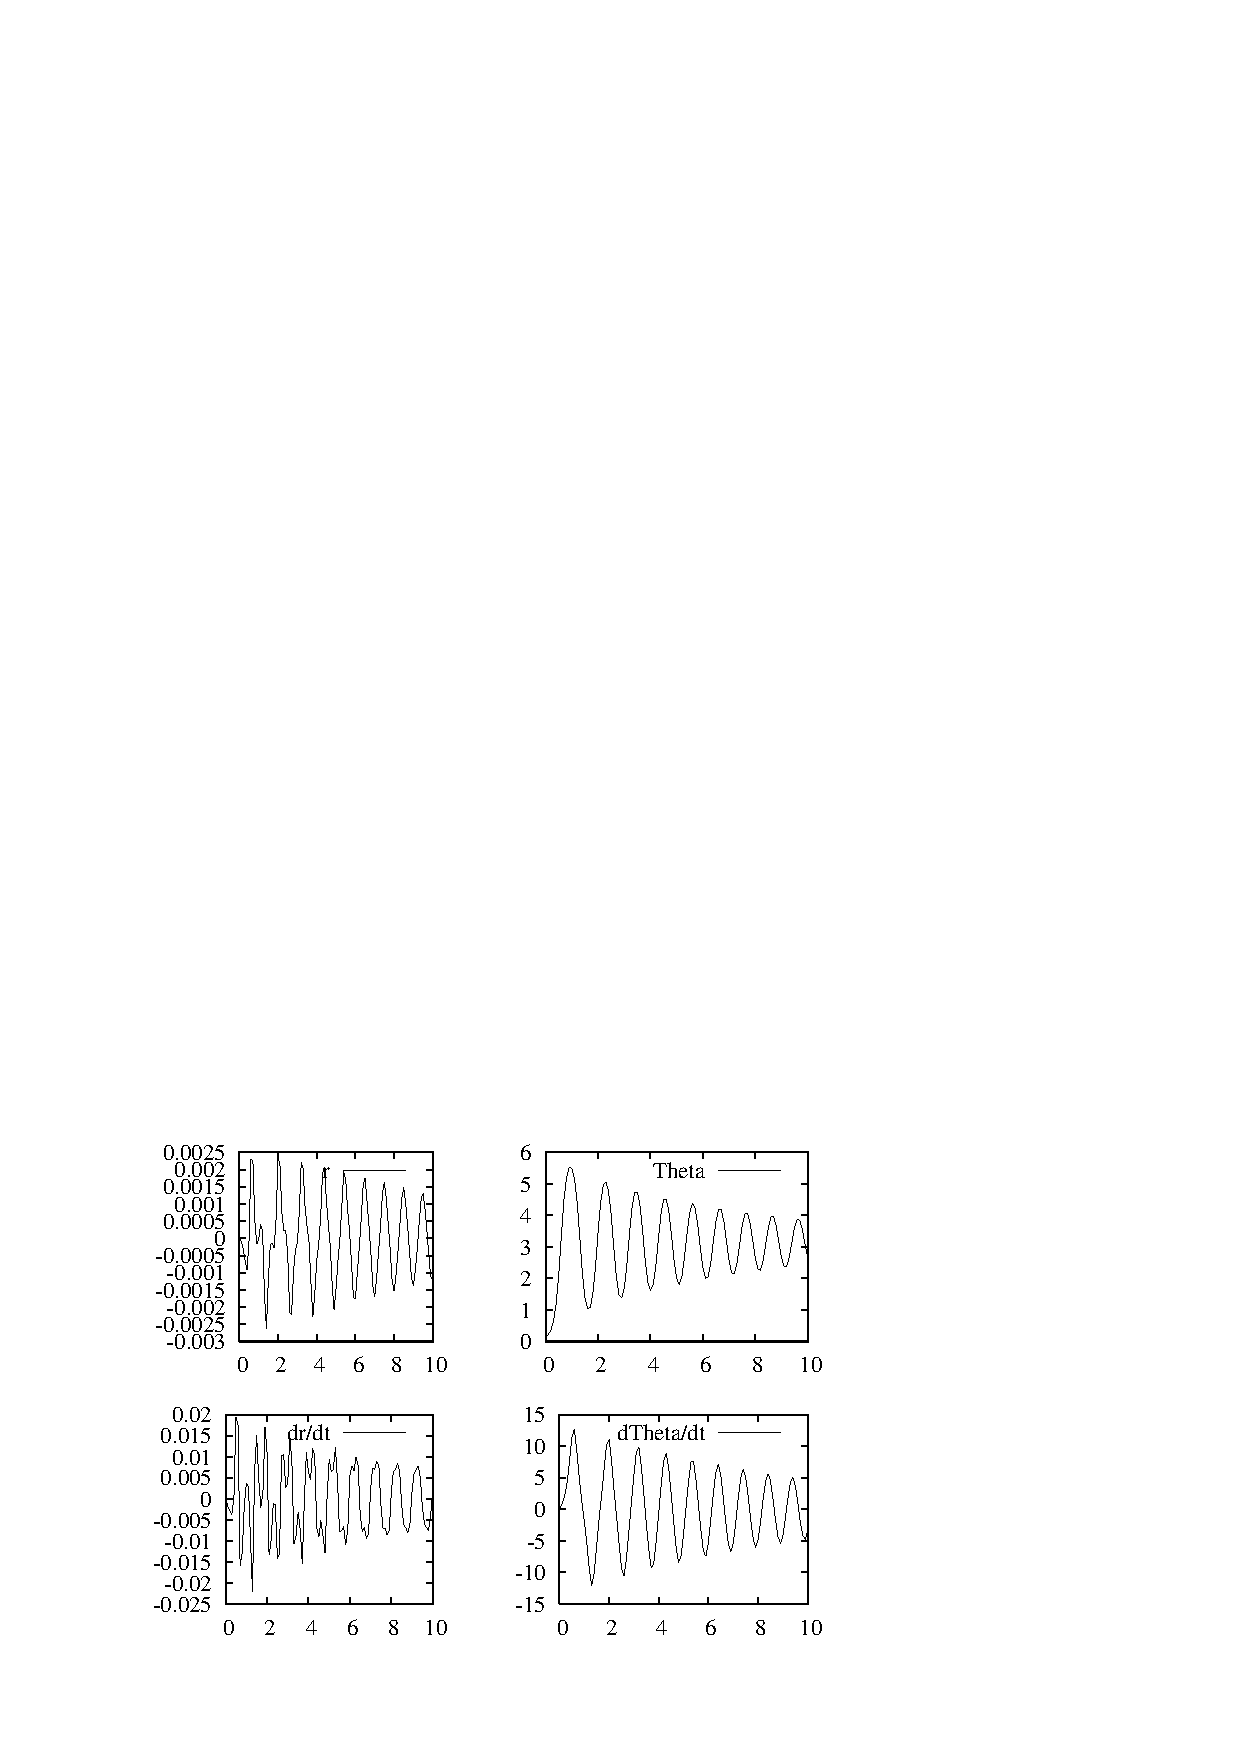
\includegraphics[width=8cm]{gazo/InPeAboveNonLiner.pdf}\\
						\end{center}
						\caption{EPSファイルをPDFに変換した結果}
					\end{figure}
				
				{\large\item グラフをプリンタに出力する}\\
				
					上で変換したPDFファイルを印刷した。\\
				
				{\large\item 関数Odeの代わりにOde45やOde45Autoを用い、結果を比較する}\\
				
				まず、Odeで計算した結果とOde45で計算した結果を比較する。以下にOdeで計算した場合とOde45で計算した場合を一緒
				のグラフにプロットした図を示す。\\
				\begin{figure}[htbp]
					\begin{center}
						\includegraphics[width=8cm]{gazo/OdeOde45Comp.pdf}\\
					\end{center}
					\caption{Odeを使用した場合とOde45を使用した場合の比較}
				\end{figure}
				\\
				関数Odeは微分方程式をルンゲ・クッタ法で求める方法であり関数Ode45は微分方程式をRunge-Kutta-Fehlberg(RKF45)
				で求める方法である。つまり、両関数は微分方程式の解法が異なるだけである。図5からは両関数における大きな違いを確認
				することはできない。\\
				次にOdeで計算した結果とOde45Autoで計算した結果を比較する。以下にOdeで計算した場合とOde45Autoで計算した場合
				を一緒にのグラフにプロットした図を示す。
				\begin{figure}[htbp]
					\begin{center}
						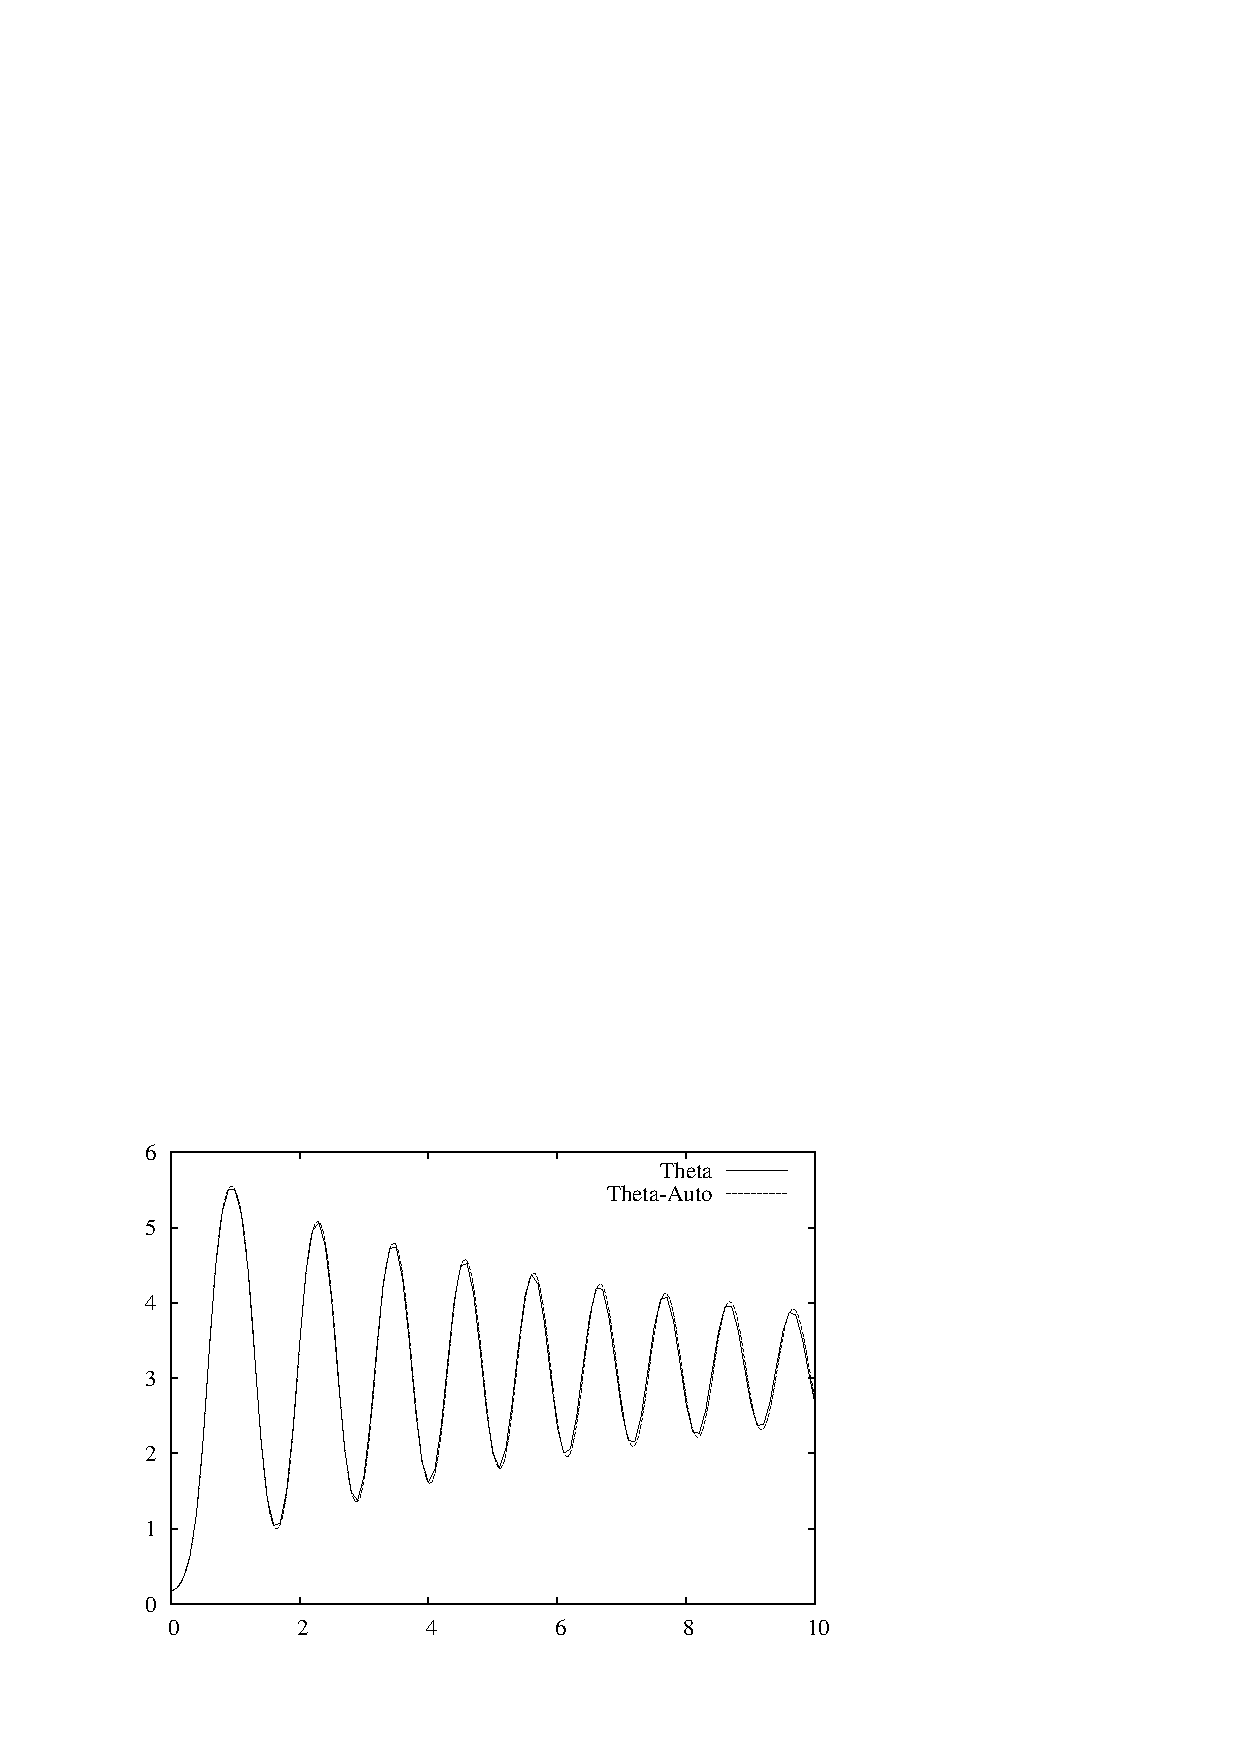
\includegraphics[width=8cm]{gazo/OdeOde45AutoComp.pdf}\\
					\end{center}
					\caption{Odeを使用した場合とOde45Autoを使用した場合の比較}
				\end{figure}
				\\
				Ode45Autoを用いることで変化が急なところの描画がより滑らかになっていることが確認できる。Ode45Autoは応答の緩急に応じ
				て刻み幅を自動で調整してくれる関数である。\\
				
				
			\end{enumerate}
			{\Large\item 線形モデルに基づくシミュレーションおよび非線形モデルとの比較}\\
			\begin{enumerate}
				{\large\item 倒立振子の非線形モデルと線形モデルの自由応答を比較する}\\
				
					最初に線形モデルのdiff$\_$eqs()を以下に示す。\\
					\begin{itembox}[l]{diff\_eqs()}
						// diff\_eqs() は微分方程式を記述する関数\\
						Func void diff\_eqs(DX,t,X,UY)\\
						// tは時間\\
						Real t;\\
						Matrix X,DX,UY;\\
						\{\\
							Real M,m,l,J,f,a,c,g;\\
							Matrix xp,up,dxp;\\\
							Matrix A,B,A21,A22,B2,K;\\
						\\
							//物理パラメータの設定\\
							M=1.49;        m=0.038; l=0.13;\\
							J=4.5E-4; f=15.10; a=0.73;\\
							c=2.1E-4; g=9.8;\\
							\\
							K=[[M+m,m*l][m*l,J+m*l\^2]];\\
							A21 = K~*[[0,0][0,m*g*l]];	\\
							A22 = K~*[[-f,0][0,-c]];\\
							A=[[Z(2),I(2)][A21,A22]];\\
							\\
							B2 = K~*[[a][0]];\\
							B=[[Z(2,1)][B2]];\\
							\\
							//Xはx=(r Theta dr/dt dTheta/dt)\^Tを表す\\
							xp = X;\\
							// Uyは入力\\
							up = UY;\\
							\\
							dxp = A*xp+B*up;\\
							\\
							DX = [dxp];\\
							\\
						\}\\
					\end{itembox}
					\\
					以下に上の線形モデルを用いて出力したデータのプロットと非線形モデルを用いて出力したデータのプロットを比較した図を
					示す。\\
					\begin{figure}[htbp]
					\begin{center}
						\includegraphics[width=8cm]{gazo/InPeAboveLiner.pdf}\\
					\end{center}
					\caption{線形モデルの出力データ}
					\end{figure}
					\begin{figure}[htbp]
					\begin{center}
						\includegraphics[width=8cm]{gazo/AboveLinerNonLinerComp.pdf}\\
					\end{center}
					\caption{線形モデルと非線形モデルの比較}
					\end{figure}
					\\
					図8はほとんど非線形モデルのグラフしか見えないが、線形モデルは0秒付近においてのみ描画されている。\\
					図7からこの線形モデルの応答が発散していることがわかる。つまり、この線形モデルではうまくいかないことがわかる。\\
				
				{\large\item 時間が進むにつれ、応答がますます離れていくのはなぜか?安定性について調べよ}\\
				
					$\theta$を微小範囲内で考えたためである。振子を上から$10^{゜}$ずらして手を離した場合、振子は真っ逆さまにおいて
					いき、$\theta$は大きくなり、前提としている$\theta$を微小範囲内という条件を満たさなくなってしまう。このような平衡点を
					不安定平衡点という。また、固有値を調べてその実部を見ることでそのモデルの安定性を調べることができる。今回の振子が上
					向き線形モデルの固有値$\lambda$はMaTXのeigval関数を用いると\\
					\begin{equation}
						\lambda = \left[
						\begin{array}{c}
							0\\
							0\\
							0.87\\
							-4.3\\
						\end{array}
						\right]
					\end{equation}
					となった。このときすべての極の実部が負でないので安定でないことがわかる。\\
					
				
				{\large\item 振り子の角度を鉛直下向を$\theta=0$として、状態方程式を求める}\\
				
					このとき、	(14)、(15)式は振子が上向きであるときを$\theta=0$として設定している。ここでは、振子が下向きであるときを
					$\theta=0$として設定しているので、(14),(15)式の三角関数内の$\theta$に+$\pi$すれば求めたい状態方程式を導くこ
					とができるといえる。なので、振り子の角度を鉛直下向きを$\theta=0$としたときの状態方程式は\\
					\begin{equation}
						\dot{x} = f(x,u)=\left[
						\begin{array}{ccc}
							\dot{r}\\
							\dot{\theta}\\
							K^{-1}\left[
							\begin{array}{ccc}
								-f\dot{r}-ml\ddot{\theta}\sin{\theta}+au\\
								-mgl\sin{\theta}-c\dot{\theta}
							\end{array}
							\right]
						\end{array}
						\right]
					\end{equation}
					\\
					となる。ただし、$K$は
					\begin{equation}
					K=\left[
					\begin{array}{ccc}
						M+m & -ml\cos{\theta}\\
						-ml\cos{\theta} & J+ml^{2}\\
					\end{array}
					\right]
					\end{equation}
				
				{\large\item 平衡点$x=\begin{pmatrix} 0 & 0 & 0 & 0 \end{pmatrix}^{\mathrm{T}}$近傍で線形化し、(線形モデル)線形
				状態方程式$\dot{x}=Ax+Bu$と出力方程式$y=Cx$を導く。}\\
				
					振子の角度を鉛直上向きを$\theta=0$としたときの状態方程式を線形化したときと同様に(29),(30)式を線形化すると
					線形状態方程式は\\
					\[\dot{x}=A\textgt{x}+B\textgt{u}\]
					\begin{equation}
						=\left[
						\begin{array}{cccc}
							0 & 0 & 1 & 0 \\
							0 & 0 & 0 & 1 \\
							0 & 0 & K^{'-1}(-f) & 0 \\
							0 & K^{'-1}(-mgl) & 0 & K^{'-1}(-c)\\
						\end{array}
						\right]
						\left[
						\begin{array}{c}
							r\\
							\theta\\
							\dot{r}\\
							\dot{\theta}\\
						\end{array}
						\right] + 
						\left[
						\begin{array}{c}
							0\\
							0\\
							K^{'-1}au\\
							0\\
						\end{array}
						\right]
					\end{equation}
					\\
					となる。ただし、$K$は、
					\begin{equation}
					K=\left[
					\begin{array}{ccc}
						M+m & -ml\\
						-ml & J+ml^{2}\\
					\end{array}
					\right]
					\end{equation}
					である。\\
					また、線形出力方程式は(27)式と同様である。\\
					今後、倒立振子のシミュレーションや検証を行う際のモデルは(31),(32)式を用いる。\\
				
				{\large\item 入力を0とし、真下から$(0^\circ~20^\circ)$傾けたところから離した場合の線形モデルと非線形モデルの応答を
				比較する}\\
				
					以下に真下から$10^\circ$傾けたところから離した場合の線形モデルと非線形モデルの$\theta$の応答を比較した図を
					示す。\\
					\begin{figure}[htbp]
						\begin{center}
							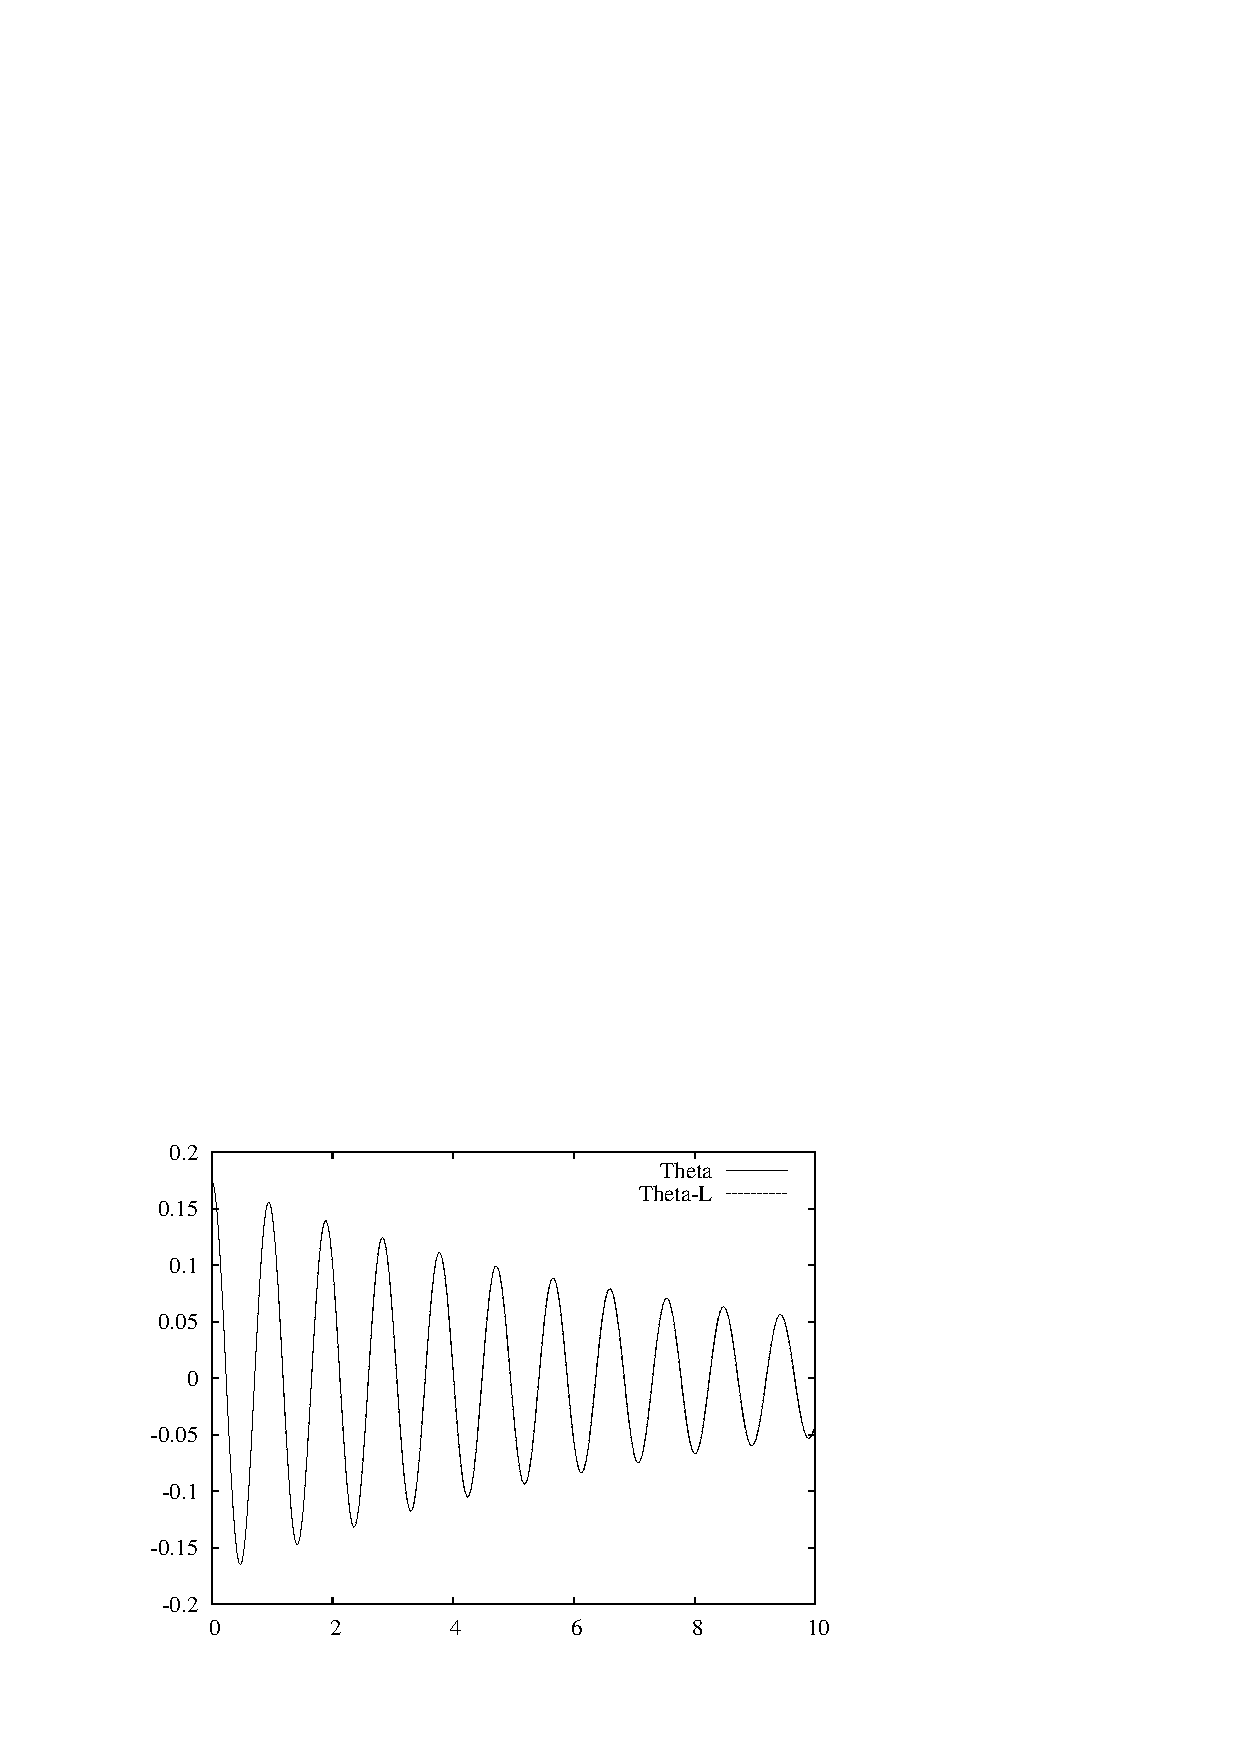
\includegraphics[width=8cm]{gazo/UnderLinerCompTheta.pdf}\\
						\end{center}
						\caption{線形モデルと非線形モデルの応答比較}
					\end{figure}
					図9から線形モデルと非線形モデルの応答がほぼ一致していることがわかる。真上の角度を$\theta=0$としたときの線形モデルの
					応答と違い発散していないことがわかる。これは真下から$10^\circ$傾けたところで$\theta$が微小範囲から大きくなることがな
					いためである。このときの平衡点を安定平衡点という。以下の節で行うパラメータの同定、検証においてはこの線形モデルを使用
					しても問題ないことになる。\\
				
			\end{enumerate}
			{\Large\item Java(NFC)によるモデリングとシミュレーション}\\
			\begin{enumerate}
				{\large\item 準備}\\
				
				nfcとwheelsをeclipseにインストールした\\
				倒立振子のシミュレーションを実行するプロジェクトを作成した\\
				その他準備を行った上で以下の作業を行う準備がそろっている。\\
				
				{\large\item モデリングとシミュレーション}\\
				
				ここでは、先ほど終了した準備をもとにjavaを用いてシミュレーションをモデリングを行う。上で線形モデルを用いると述べたがここでは
				非線形モデルをJAVAファイルに記述することでシミュレーションを行う。\\
				シミュレーションは倒立振子システムを表すPendulumクラスとシミュレーション対象システムを生成するFreePendulumクラスとシミュレー
				ションを実行するFreePendulumSimulationクラスによって行う。以下にシミュレーションを行ってgnuplotに描画した結果を以下に示
				す。ちなみにシミュレーションは鉛直下向きを$\theta=0$として行う\\
				\begin{figure}[htbp]
					\begin{center}
						\includegraphics[width=8cm]{gazo/FreePendulumSimulationJAVAThetaR.pdf}\\
					\end{center}
					\caption{JAVAによるシミュレーション($\theta$を表示)}
				\end{figure}
				\begin{figure}[htbp]
					\begin{center}
						\includegraphics[width=8cm]{gazo/FreePendulumSimulationJAVAr.pdf}\\
					\end{center}
					\caption{JAVAによるシミュレーション($r$を表示)}
				\end{figure}
				
			\end{enumerate}
			{\Large\item Jamoxによるモデリングとシミュレーション}\\
			\begin{enumerate}
				{\large\item ユーザ定義動的システム(Java)による倒立振子システム}\\
				
					先ほど作成した倒立振子を表すPendulumクラスを用いて、JAMOXでシミュレーションを行う。\\
					以下に倒立振子のシミュレーションモデル(ブロック線図)と自由応答を示す。\\
					\begin{figure}[htbp]
					\begin{center}
						\includegraphics[width=8cm]{gazo/BlockNonLinerJ.pdf}\\
					\end{center}
					\caption{使用したブロック線図}
					\end{figure}
					\begin{figure}[htbp]
					\begin{center}
						\includegraphics[width=8cm]{gazo/FreePendulumSimulationJAMOXJ.pdf}\\
					\end{center}
					\caption{自由応答波形}
					\end{figure}
				
				
				{\large\item ユーザ定義動的システム(MaTX)による倒立振子システム}\\
					
					今度はMaTXを用いて同様のシミュレーションを行う。以下に倒立振子のシミュレーションモデル(ブロック線図)と自由応答波形
					を示す。\\
					\begin{figure}[htbp]
					\begin{center}
						\includegraphics[width=8cm]{gazo/BlockNonLinerM.pdf}\\
					\end{center}
					\caption{使用したブロック線図}
					\end{figure}
					\begin{figure}[htbp]
					\begin{center}
						\includegraphics[width=8cm]{gazo/FreePendulumSimulationJAMOXM.pdf}\\
					\end{center}
					\caption{自由応答波形}
					\end{figure}
				
			\end{enumerate}
		\end{enumerate}	

		{\LARGE\item \textgt{倒立振子のパラメータ同定と検証}}\\ 
		\begin{enumerate}
			{\Large\item 実験環境(Linux2.6 + RtMaTX)の整備と確認}\\
			\begin{enumerate}
				{\large\item 実験方法}\\
				
					実験は実験室のPCと倒立振子を使う。PCで倒立振子の計測を行うには、ディレクトリRtMaTX内に存在するSample.mmファイ
					ルを用いる。Sample.mmをコンパイルするにはシェル内でmakeと打ち、Sample.mmを実行するには sudo ./sampleと入力すれば
					よい。実行した後は$\theta$とプログラム開始時を初期値として$r$の測定画面が現れる。cを押すことで台車に入力値が入
					り、測定が開始される。\\
					
				{\large\item sample.mmの解読}\\
				
					適宜必要な時に行えばよいかと。とりあえず入力を変えたいときはオンライン関数内のactuator()の引数を変えればよい。それ以
					上の情報はここでは\\
				
			\end{enumerate}
			{\Large\item パラメータの同定}\\
			\begin{enumerate}
				{\large\item 振り子の質量mの同定}\\
				
					振り子は台車から取り外した棒の部分を振り子として扱う。つまり、台車と振り子をつなぐための直方体の物体は台車の一部と
					して扱うことにする。同定は計量器を用いた。ここで計量器の精度が有効数字二桁までしかないので以後同定したパラメータも
					有効数字二桁で扱う。以下に同定した結果を示す。
					\begin{equation}
						m=3.1E-2(kg)
					\end{equation}
				
				{\large\item 振り子の回転軸から重心までの長さlの同定}\\
				
					先ほどと同様の振り子に対して重心までの長さを同定する。(見た感じ)振り子が左右対称であることを利用して振り子のちょう
					ど真ん中の位置を定規で測定した。以下に同定した結果を示す。
					\begin{equation}
						l=1.5E-1(m)
					\end{equation}
				
				{\large\item 変位rの測定値への変換係数$c_{1}$の同定}\\
				
					最初から設定してある。
					\begin{equation}
						c_{1}=1.0(V/m)
					\end{equation}
				
				{\large\item 角度$\theta$の測定値への変換係数$c_{2}$の同定}\\
				
					最初から設定してある。
					\begin{equation}
						c_{2}=1.0(V/m)
					\end{equation}
				
				{\large\item 駆動アンプへの入力電圧から台車への駆動力までのゲインaの同定}\\
				
					詳しい同定方法は資料の方を参考にしてもらいたい。ここでは、簡単に説明する。まず台車を左の方に位置させて台車を駆動
					させる。この時台車にばねばかりをひっかけ2パターンの状況においてその値を測定する。まずは台車をばねばかりでぎりぎり動か
					ない力で引っぱった場合、次に台車をばねばかりで逆に左に動き出す力で引っ張った場合、の2パターン値を入力電圧を変えな
					がら測定していく。そして、各パターンにおいて最小二乗法を用いて一時関数を求める。この傾きをaとする。以下に同定した値
					を示す。
					\begin{equation}
						a=0.062(Kg/V) = 6.1E-1(N/V)
					\end{equation}
				
				{\large\item 重心まわりの慣性モーメントJの同定}\\
				
					振り子を自由振動させることにより、Jとcを測定できる。詳しい数式は資料を参考されたい。ここでは簡単に説明する。振り子を
					自由振動させたときのデータからグラフを描画させる。グラフにおいて一つ目の山とその次の山から減衰比を求める。また、一つ目
					の山から次の山までにかかる時間を1周期として求める。この値を利用してJとcを求める。以下にJを求めるのに使用した数式を
					示す。
					\begin{equation}
						J=\frac{mglT_{2}^{2}}{4\pi^{2}+\lambda^{2}}-ml^{2}
					\end{equation}
					(38)式よりJは以下のように同定された。
					\begin{equation}
						J=2.5E-4(khm^{2})
					\end{equation}
				
				{\large\item 回転軸摩擦係数cの同定}\\
				
					上の通りである。以下にcを求めるのに使用した数式を示す。
					\begin{equation}
						c=\frac{2\lambda(J+ml^{2})}{T_{2}}
					\end{equation}
					(40)式よりcは以下のように同定された。
					\begin{equation}
						c=5.4E-5(kgm^{2}/s)
					\end{equation}
				
				{\large\item 台車の質量Mの同定}\\
				\begin{enumerate}
					{\item ステップ応答による方法}\\
					
						振り子を台車から取り外して、台車のステップ応答を測定する。詳しい数式は資料に譲る。各電圧についてステップ応答を							測定し、グラフを描画する。そのグラフから傾きKU0とその傾きを持つ一次関数を仮定したとき$r(t)=0$となるtをTとして決定							する。KとTからMとfを決定する。以下に同定したMを示す。
						\begin{equation}
							M=6.9E-1(kg)
						\end{equation}
						
					{\item フィードバックによる方法}\\
					
						振り子を台車から取り外すのは同じ。入力がステップ応答ではなくフィードバックになるのでそこを考慮する必要がある。
						つまり、sample.mmにおいてactuator()の引数を
						\[u=k_{c}*(y_{c}-y)\]
						という風に変更しなければならない。これができれば台車は目標値に向かってフィードバックし始める。\\
						得られたデータ列をプロットし、減衰比とその周期(Jとcの同定で用いた方法と同じ)を求める。
						求めたJとcから以下の式を用いて$\zeta$と$\omega_{n}$を計算し求める。
						\begin{equation}
							\lambda=\frac{2\pi\zeta}{\sqrt{1-\zeta^{2}}}
						\end{equation}
						\begin{equation}
							T_{2}=\frac{2\pi}{\omega_{n}\sqrt{1-\zeta^{2}}}
						\end{equation}
						上の式を式変形して$\zeta$と$\omega_{n}$イコールの式にすると
						\begin{equation}
							\zeta=\frac{\lambda}{\sqrt{4\pi^{2}+\lambda^{2}}}
						\end{equation}
						\begin{equation}
							\omega_{n}=\frac{2\pi}{T_{2}\sqrt{1-\zeta^{2}}}
						\end{equation}
						以上の式から求めた$\zeta$と$\omega_{n}$は以下の二次系の伝達関数の基本形に代入することで
						実験で得られたデータから伝達関数を求めることができる
						\begin{equation}
							G(s) = \frac{\omega_{n}^{2}}{s^{2}+2\zeta\omega_{n}s + \omega_{n}^{2}}
						\end{equation}
						また、今回のフィードバック制御系におけるブロック線図は以下のようになる。
						\begin{figure}[htbp]
						\begin{center}
							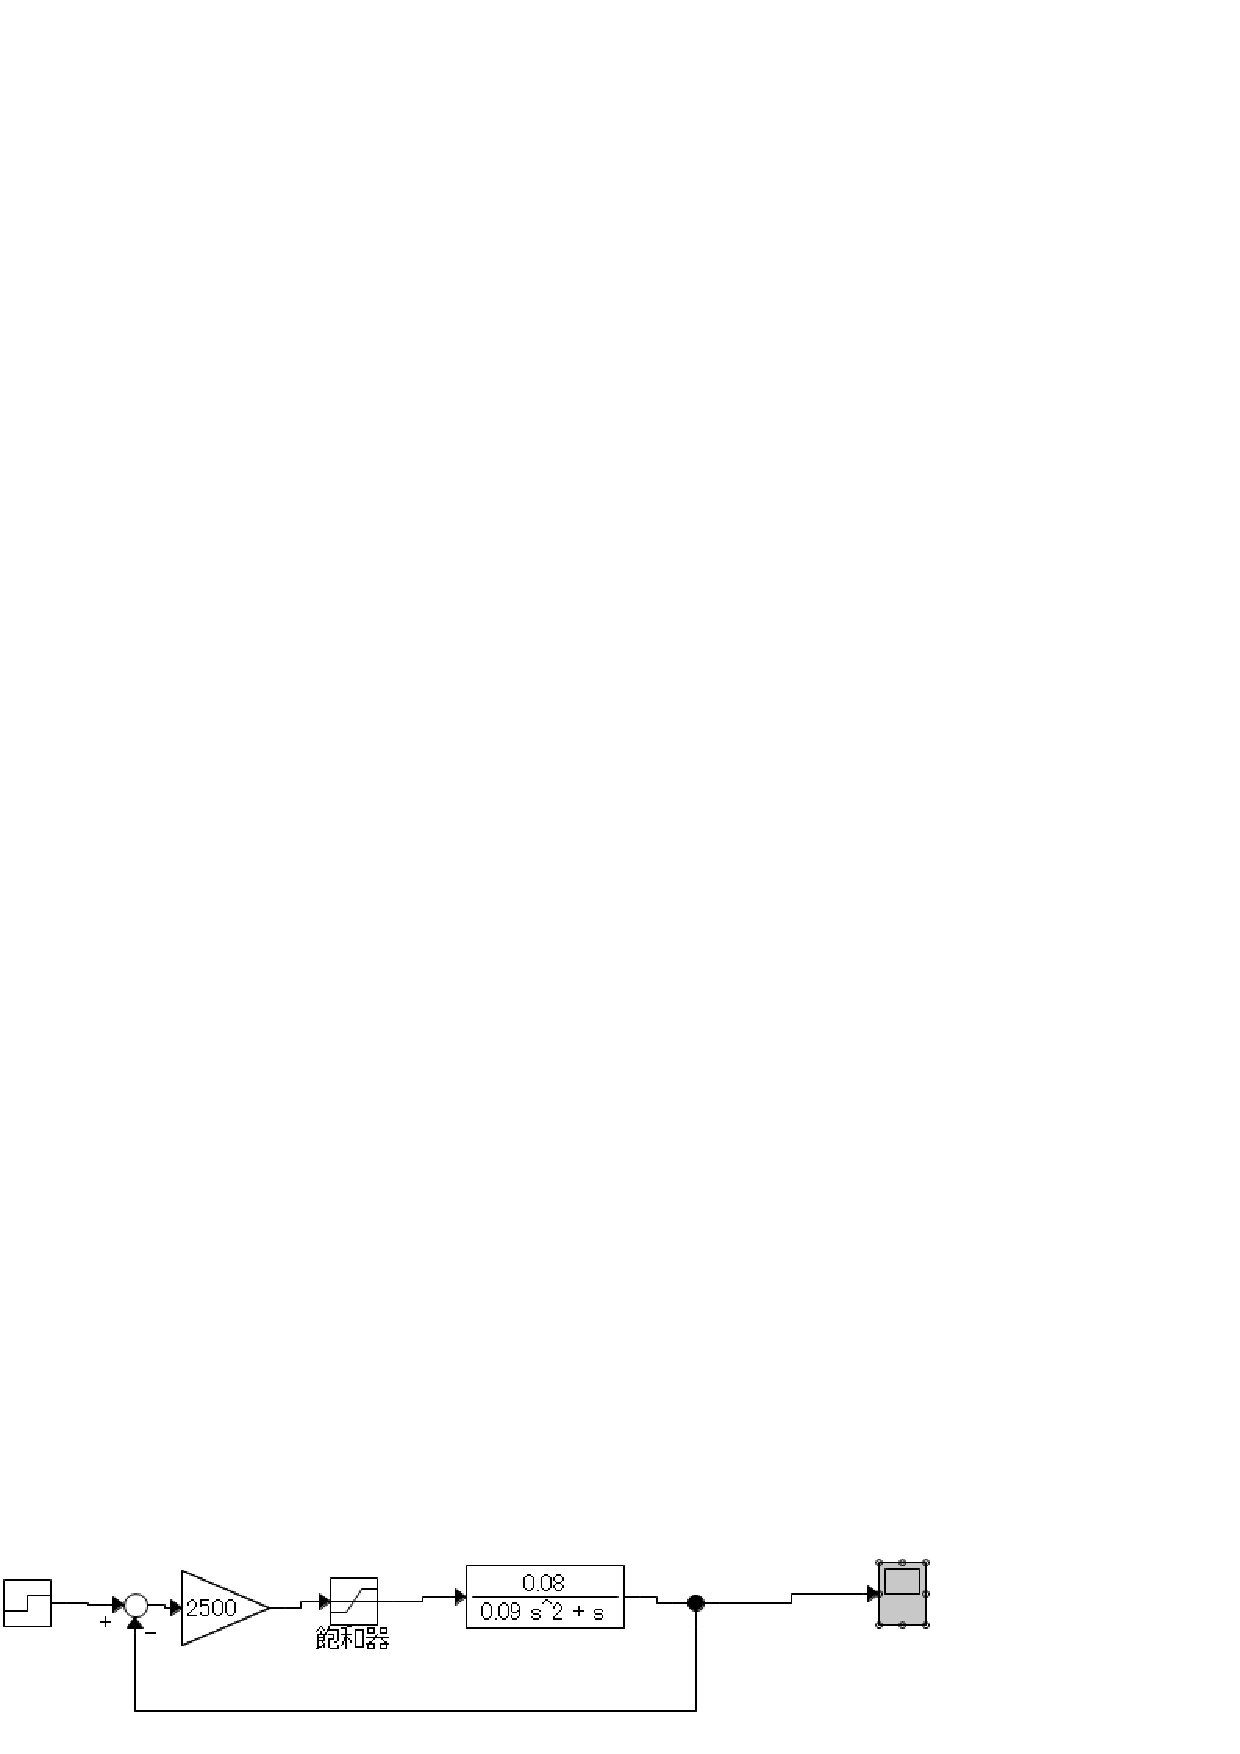
\includegraphics[width=8cm]{gazo/FeedBackCart.pdf}\\
						\end{center}
						\caption{フィードバック制御系のブロック線図}
						\end{figure}
						ここで、台車の伝達関数は以下の式である。
						\begin{equation}
							P(s)=\frac{K}{s(Ts+1)}
						\end{equation}
						ただし、Tは$M/f$、Kは$a/f$である。上のブロック線図から伝達関数を求める。
						しかし、飽和システムを含んでいると伝達関数を求めることができないので、ここでは飽和システムがなくても
						台車は問題なく動作するもとして仮定する。以上の仮定から伝達関数は
						\begin{equation}
							G(s) = \frac{AK/T}{s^{2}+(1/T)s+(AK/T)}
						\end{equation}
						となる。ただしAはゲインである。(47)式と(49)式を係数比較し、M、f=の式にすると以下のようになる。
						\begin{equation}
							\left\{
							\begin{array}{l}
								M=\frac{aA}{\omega_{n}^{2}} \\
								f=2\zeta\omega_{n}^{2}M
							\end{array}
							\right.
						\end{equation}
						よって、(50)式からMとfは以下のように求まる。
						\begin{equation}
						\left\{
						\begin{array}{l}
							M=1.59(kg)\\
							f=13.2(kg/s)
						\end{array}
						\right.
						\end{equation}
											
					{\item 2つの方法で求めたパラメータを比較する。パラメータが異な場合、その理由を考察する。}\\
					
						(42),(52)式と(51)式を比べるとまるで違うことがわかる。
						考察:結論から述べると飽和システムを無視しても問題なく動作すると仮定してパラメータを計算したためである。\\
						飽和システムを無視したことによる差異が生まれる\\
						飽和システムは飽和システムに設定した以上の電圧が入ったときにそのオーバーした分をカットする
						つまり飽和システムを無視することによりカットするかしないかで差異が生まれる
						実際に飽和システムにかかる前の電圧をシミュレーションとしてJAMOXか何かで見てみるといいが収束値0.2でゲイン250
						のとき一番最初に入力される電圧はなんと500Vである。これがどのくらいの電圧なのか専門家でないので知る余地もないが
						これを15Vとみなすかみなさないかで大きく差異が生まれるといえるだろう。画像は各自でそろえてほしい。mendoi
						なら飽和システムを含めて伝達関数を求めればよいのではないか?\\
						→飽和システムを含んでいるブロック線図の伝達関数は求めることができない(線形システムでないため)\\
						なら飽和システムに設定した以上の電圧が入らないように収束値、ゲインを調整すればよいのではない?\\
						→0.2に収束させるという条件で15Vを超えないゲインはだいたい70に設定すればよい。\\
 						だがこれではツェータが1を超えてしまいオーバーシュートしなくなる。つまりゲイン操作によって15V以内に入力を抑えるこ
 						とは不可能\\
						→ゲイン1500という設定で15Vを超えないような収束値は0.01である。つまり台車を1cmだけ動かすことになる。
						ハード的な問題から収束値1cmで正確なデータが取れるとは思えない\\

						つまり、以上から本実験においてフィードバックを行う場合必ず飽和システムが必要であるといえる。
						なので、飽和システムが存在する限り伝達関数を求めることができないので、正確なパラメータの計算を行うことができないと
						いえる。
						考察終わりん子
					
				\end{enumerate}
				{\large\item 台車の摩擦係数fの同定}\\
				
					上に示した通りである。ただし、ここではステップ応答による方法のみ取り扱う。以下に同定した値を示す。
					\begin{equation}
						f=7.6(kg/s)
					\end{equation}
				
				{\large\item パラメータを表にまとめる}\\
				
					同定実験において同定したパラメータを表にまとめる。\\
					\\
					\begin{tabular}{|c|c|}\hline
						パラメータ & 同定した値 \\ \hline\hline
						m[kg]  & 0.031\\ \hline
						l[m] & 0.15\\ \hline
						M[kg] & 0.69\\ \hline
						f[kg/s] & 7.56\\ \hline
						J[$kgm^{2}$] & 2.5E-4\\ \hline
						c[$kgm^{2}/s$] & 5.4E-5\\ \hline
						a[N/V] & 0.61\\ \hline
						$c_{1}$[V/m] & 1.0\\ \hline
						$c_{2}$[V/m] & 1.0\\ \hline
					\end{tabular}
					
				
			\end{enumerate}
			{\Large\item パラメータの検証}\\
			\begin{enumerate}
				{\large\item 台車のステップ応答}\\
				\begin{enumerate}
					{\item MaTXによる}\\
					
						以下に実験データとシミュレーション結果を重ね合わせたグラフを示す。ただし、入力電圧を8Vのときである。
						\begin{figure}[htbp]
						\begin{center}
							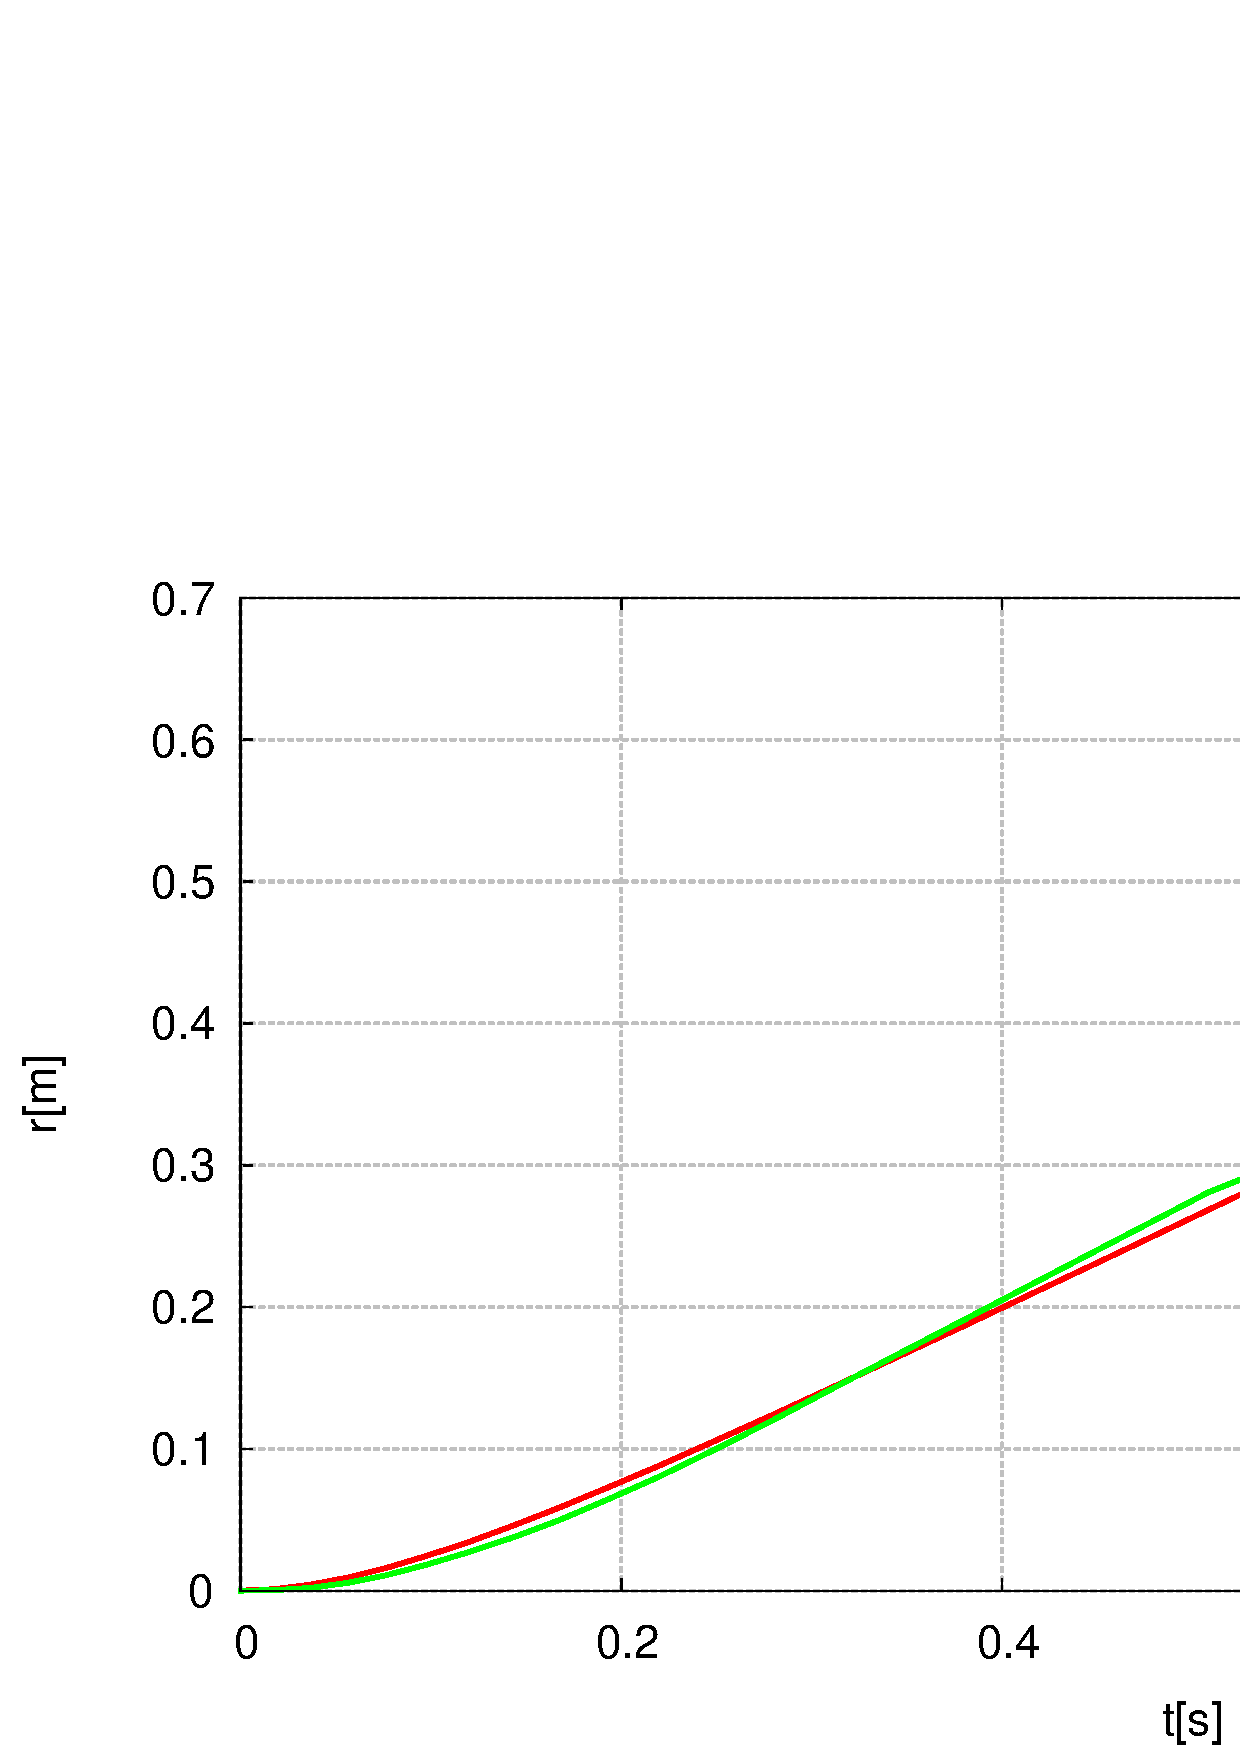
\includegraphics[width=8cm]{gazo/nabe8.pdf}\\
						\end{center}
						\caption{ステップ応答の実験データとシミュレーション結果のグラフ(MaTX)}
						\end{figure}
						
					{\item Javaによる}\\
					
						以下にjavaを用いて実験データとシミュレーション結果を重ね合わせたグラフを示す。ただし、入力電圧は8Vである。
						\begin{figure}[htbp]
						\begin{center}
							\includegraphics[width=8cm]{gazo/nabe8StepJAVA.pdf}\\
						\end{center}
						\caption{ステップ応答の実験データとシミュレーション結果のグラフ(JAVA)}
						\end{figure}
					
					{\item Jamoxによる}\\
					
						以下にJAMOXを用いて実験データをシミュレーション結果を重ねたグラフを示す。ただし、入力電圧は8Vである。
						ブロック線図は省略する。
						以下にユーザー定義関数システムJAVAを用いて検証した結果を示す。
						\begin{figure}[htbp]
						\begin{center}
							\includegraphics[width=8cm]{gazo/StepCartJAMOXJ.pdf}\\
						\end{center}
						\caption{ステップ応答の実験データとシミュレーション結果のグラフ(JAMOX(JAVA))}
						\end{figure}
						以下にユーザー定義関数システムMATXを用いて検証した結果を示す。
						\begin{figure}[htbp]
						\begin{center}
							\includegraphics[width=8cm]{gazo/StepCartJAMOXM.pdf}\\
						\end{center}
						\caption{ステップ応答の実験データとシミュレーション結果のグラフ(JAMOX(MATX))}
						\end{figure}
						
					
				\end{enumerate}
				{\large\item 台車のフィードバック応答}\\
				\begin{enumerate}
					{\item MaTXによる}\\
					
						以下にmatxを用いて実験データとシミュレーション結果を重ね合わせたグラフを示す。ただし、使用したMとfは
						ステップ応答によって求めたMとfを用いる。また、ゲインは1500に設定した。
						\begin{figure}[htbp]
						\begin{center}
							\includegraphics[width=8cm]{gazo/FreeBackCartOldParaMATX.pdf}\\
						\end{center}
						\caption{フィードバック応答の実験データとシミュレーション結果のグラフ(MATX)}
						\end{figure}
					
					{\item Javaによる}\\
					
						以下にjavaを用いて実験データとシミュレーション結果を重ね合わせたグラフを示す。ただし、使用したMとfは
						フィードバック応答によって求めたMとfを用いている。
						\begin{figure}[htbp]
						\begin{center}
							\includegraphics[width=8cm]{gazo/FeedBackCompwithFeedBackParaJAVA.pdf}\\
						\end{center}
						\caption{フィードバック応答の実験データとシミュレーション結果のグラフ(新しいパラメータ)(JAVA)}
						\end{figure}
						この方法で求めたパラメータではうまくいかないという結論を出したのでパラメータを戻して再びグラフをプロットして見る。
						ただし、ゲインは1500に設定した。
						\begin{figure}[htbp]
						\begin{center}
							\includegraphics[width=8cm]{gazo/FeedBackCartOldPatraJAVA.pdf}\\
						\end{center}
						\caption{フィードバック応答の実験データとシミュレーション結果のグラフ(JAVA)}
						\end{figure}
						
					
					{\item Jamoxによる}\\
						
						以下にJAMOXを用いて実験データをシミュレーション結果を重ねたグラフを示す。ただし、Mとfは
						ステップ応答によって求めた値を用いる。また、ゲインは1500に設定した。
						以下にユーザー定義関数システムJAVAを用いて検証した結果を示す。
						\begin{figure}[htbp]
						\begin{center}
							\includegraphics[width=8cm]{gazo/FeedBackCartOldParaJAMOXJ.pdf}\\
						\end{center}
						\caption{ステップ応答の実験データとシミュレーション結果のグラフ(JAMOX(JAVA))}
						\end{figure}
						以下にユーザー定義関数システムMATXを用いて検証した結果を示す。
						\begin{figure}[htbp]
						\begin{center}
							\includegraphics[width=8cm]{gazo/FeedBackCartOldParaJAMOXM.pdf}\\
						\end{center}
						\caption{ステップ応答の実験データとシミュレーション結果のグラフ(JAMOX(MATX))}
						\end{figure}
					
				\end{enumerate}
				{\large\item 振り子の自由振動}\\
				\begin{enumerate}
					{\item MaTXによる}\\
					
						以下に実験データとシミュレーション結果を重ね合わせたグラフを示す。
						\begin{figure}[htbp]
						\begin{center}
							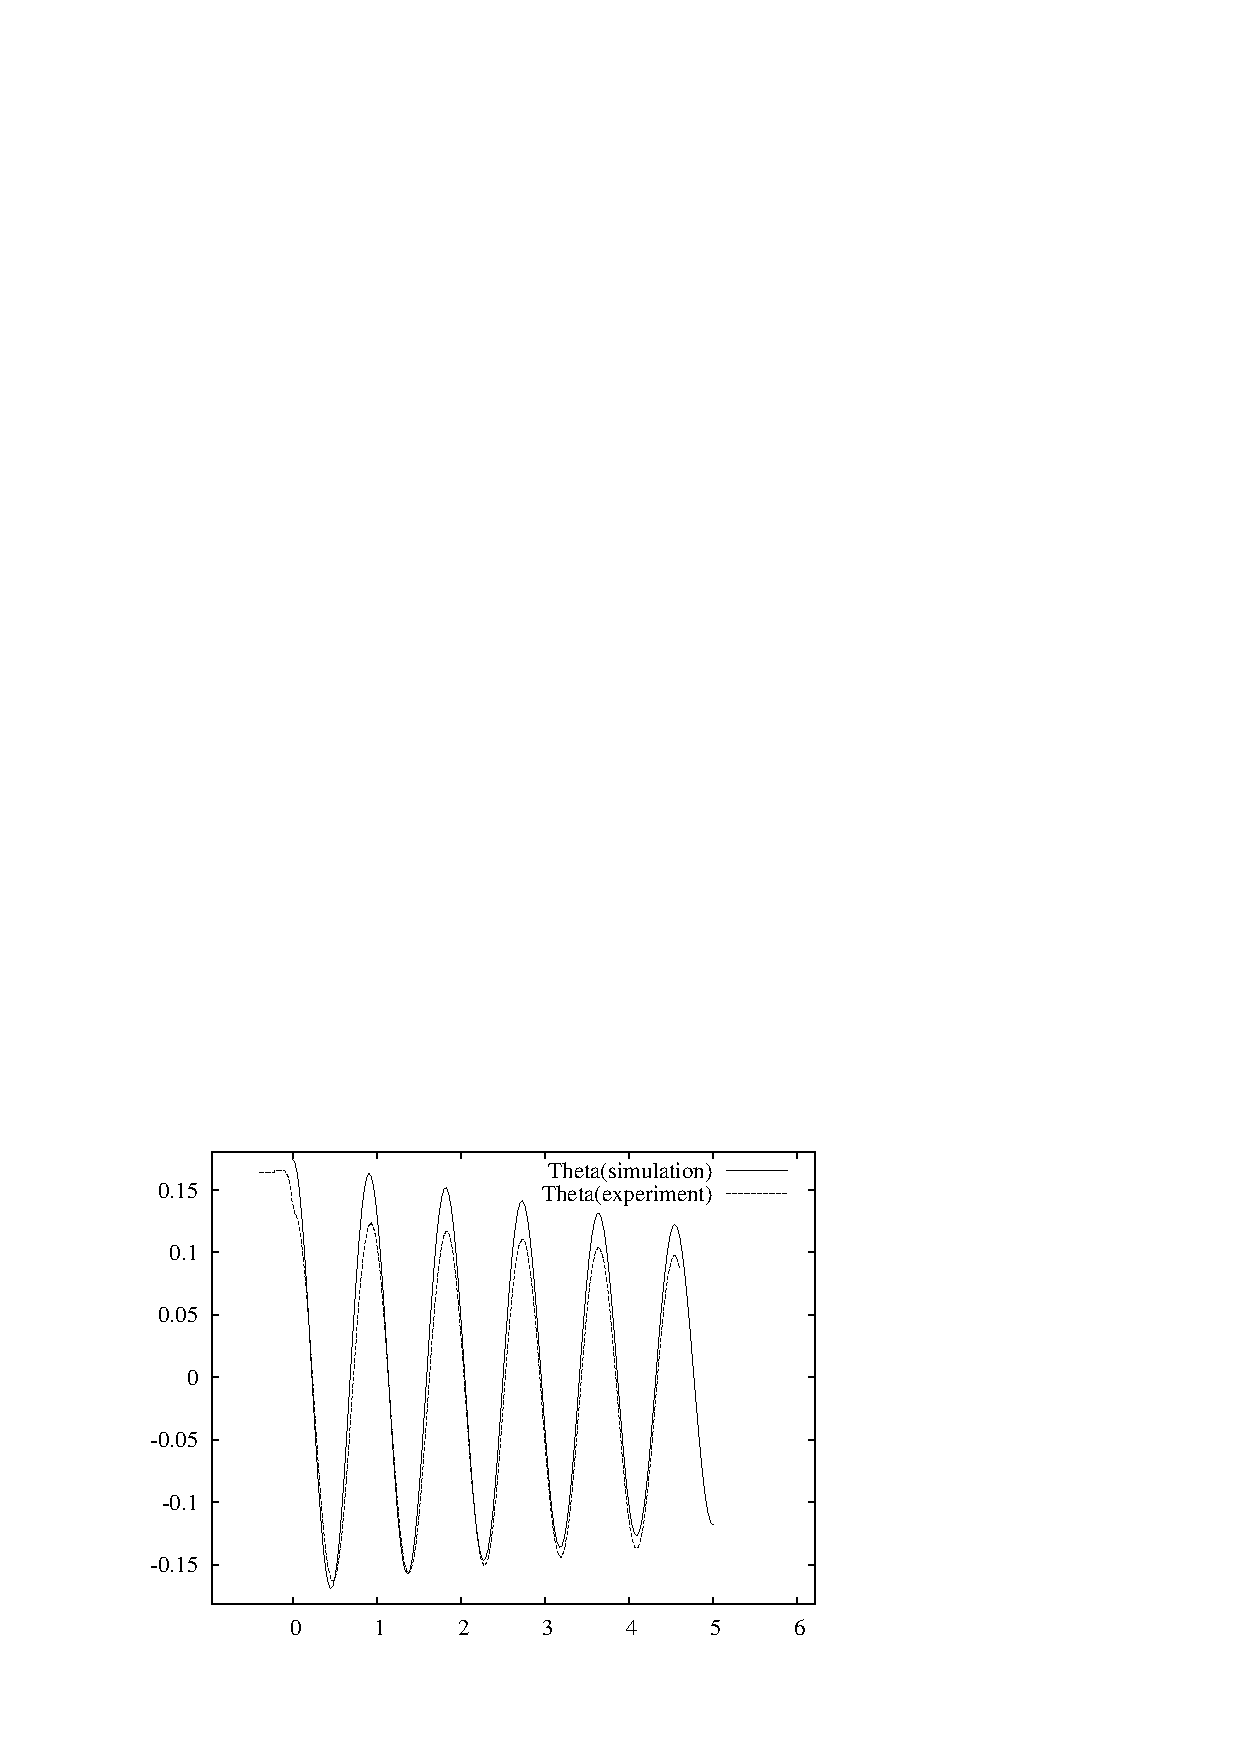
\includegraphics[width=8cm]{gazo/free45Auto.pdf}\\
						\end{center}
						\caption{自由振動の実験データとシミュレーション結果のグラフ(MaTX)}
						\end{figure}
					
					{\item Javaによる}\\
					
						以下に実験データとシミュレーション結果を重ね合わせたグラフを示す。
						\begin{figure}[htbp]
						\begin{center}
							\includegraphics[width=8cm]{gazo/freeJAVA.pdf}\\
						\end{center}
						\caption{自由振動の実験データとシミュレーション結果のグラフ(Java)}
						\end{figure}	
					
					{\item Jamoxによる}\\
					
						以下に実験データとシミュレーション結果を重ね合わせたグラフを示す。
						まずはユーザー定義動的システムJAVAを用いた場合。
						\begin{figure}[htbp]
						\begin{center}
							\includegraphics[width=8cm]{gazo/FreePendulumSimulationJAMOXJverifi.pdf}\\
						\end{center}
						\caption{自由振動の実験データとシミュレーション結果のグラフ(JAMMOX(JAVA))}
						\end{figure}
						次にユーザー定義動的システムMATXを用いた場合。
						\begin{figure}[htbp]
						\begin{center}
							\includegraphics[width=8cm]{gazo/FreePendulumSimulationJAMOXMverifi.pdf}\\
						\end{center}
						\caption{自由振動の実験データとシミュレーション結果のグラフ(JAMMOX(MATX))}
						\end{figure}
					
				\end{enumerate}
			\end{enumerate}
		\end{enumerate}

		{\LARGE\item \textgt{設計(線形)モデルの決定とシステム解析}}\\
		\begin{enumerate}
			{\Large\item MaTXによるシステム解析}\\
			\begin{enumerate}
				{\large\item 倒立振子の線形モデル(状態空間表現のA,B,Cの数値)を導き、安定性を調べる}\\
				
					ここでは上向き線形モデルを用いる。最終的には振子を制御によって立たせたいので上向きのモデルを用いて
					システム解析を行う。また、ここで線形モデルを用いるのは非線形モデルではシステム解析を行うことが
					できないためである。以下に結果を示す\\
					\\
					MaTXで計算した行列A、B、Cを以下に示す。\\
					\begin{equation}
						A=\left[
						\begin{array}{cccc}
							0 & 0 & 1 & 0 \\
							0 & 0 & 0 & 1 \\
							0 & -0.32 & -10.9 & 0.00038 \\
							0 & 50 & 53 & -0.059 \\
						\end{array}
						\right]
					\end{equation}
					\begin{equation}
						B=\left[
						\begin{array}{c}
							0 \\
							0 \\
							0.87 \\
							-4.3 \\
						\end{array}
						\right]
					\end{equation}
					\begin{equation}
						C=\left[
						\begin{array}{cccc}
							1 & 0 & 0 & 0 \\
							0 & 1 & 0 & 0 \\
						\end{array}
						\right]
					\end{equation}
					次に、システムの極(Aの固有値)を計算し、安定性を調べる。このとき、すべての極の実部が負であれば、
					安定といえる。以下にシステムの極を計算した行列Dを示す。
					\begin{equation}
						D=\left[
						\begin{array}{c}
							7.0+0i\\
							0+0i \\
							-6.8-0i \\
							-11+0i\\
						\end{array}
						\right]
					\end{equation}
					1行目は不安定、二行目は安定限界であり、他の行は安定であることがわかる。\\	
				
				{\large\item 可制御性行列のランクを計算し、可制御性を調べる}\\
				
					可制御性行列は以下のようになる。
					\begin{equation}
					N_{c} = \left[
						\begin{array}{cccc}
							C & CA & CA^{2} & CA^{3} \\
						\end{array}
						\right]
					\end{equation}
					上の行列よりランクは4になれば可制御性があるといえる。ランクを計算したところ
					\begin{equation}
						rank  = 4
					\end{equation}
					となった。よって可制御性を確認できる。\\
					
				{\large\item 可観測性行列のランクを計算し、可観測性を調べる}\\
				
					可観測性行列は以下のようになる。
					\begin{equation}
					N_{o} = \left[
						\begin{array}{c}
							C\\
							CA\\
							CA^{2}\\
							CA^{3}\\
						\end{array}
						\right]
					\end{equation}
					上の行列よりランクは4になれば可観測性があるといえる。ランクを計算したところ
					\begin{equation}
						rank = 4
					\end{equation}
					となった。よって、可観測性を確認できる。\\
					\\
					以上から倒立振子系の上向き線形モデルは不安定なシステムであるが、4つの状態を観測することができ、
					制御することが可能なシステムといえる。次の節でいよいよ倒立振子を絶たせるための制御器を設計していく。
					その際にここで計算したシステム行列Aと入力行列Bを用いる。
				
			\end{enumerate}
			{\Large\item Java(NFC)によるシステム解析}\\
			\begin{enumerate}
				{\large\item 倒立振子の線形モデル(状態空間表現のA,B,Cの数値)を導き、、安定性を調べる}\\
				
					Javaで計算した場合もMaTXで計算した場合とも全く同じになりました。\\
					なので省略いたしますことをご了承承り等ございまするようお願い申しあげ賜ります。\\
				
				{\large\item 可制御性行列のランクを計算し、可制御性を調べる}\\
				
					可制御性行列についてはMaTXの節で説明したのでここではランクについてのみ述べる。\\
					状況は同じくランクは4となればよい。ランクを計算したところ
					\begin{equation}
						rank = 4
					\end{equation}
					となった。よって、可制御性を確認できる。\\
				
				{\large\item 可観測性行列のランクを計算し、可観測性を調べる}\\
				
					もっと省く
					\begin{equation}
						rank = 4
					\end{equation}
					よって、可観測性を確認できる。\\
				
			\end{enumerate}
			{\Large\item Jamox(ユーザー定義関数java)によるシステム解析}\\
			\begin{enumerate}
				{\large\item 倒立振子の線形モデル(状態空間表現のA,B,Cの数値)を導き、、安定性を調べる}\\
				
					上に同じ結果\\
				
				{\large\item 可制御性行列のランクを計算し、可制御性を調べる}\\
				
					上に同じ結果\\
				
				{\large\item 可観測性行列のランクを計算し、可観測性を調べる}\\
				
					上に同じ結果\\
				
			\end{enumerate}
			{\Large\item Jamox(ユーザー定義関数MaTX)によるシステム解析}\\
			\begin{enumerate}
				{\large\item 倒立振子の線形モデル(状態空間表現のA,B,Cの数値)を導き、、安定性を調べる}\\
				
					上に同じ結果\\
				
				{\large\item 可制御性行列のランクを計算し、可制御性を調べる}\\
				
					上に同じ結果\\
				
				{\large\item 可観測性行列のランクを計算し、可観測性を調べる}\\
				
					上に同じ結果\\
				
			\end{enumerate}
		\end{enumerate}
		{\LARGE\item \textgt{制御系の設計1(状態フィードバック)と制御性能評価}}\\
		\begin{enumerate}
			{\Large\item MaTXによる制御系設計と制御性能評価}\\
			\begin{enumerate}
				{\large\item 制御器(状態フィードバック)を設計する。}\\
				
					ここでは線形制御器をもちいて非線形システムを制御することを目的としている。
					また、振子を上向きに配置し倒れないことも目的の一つである。
					ここで注意したいのは前に求めた線形システムを用いないことである。線形システムはそのモデルが完成している
					(極がわかっている)ので線形システムに対して制御器を設計するシミュレーションは行わなくてもよい。
					(ただし、台車の可動範囲などを狭めているという意味でシミュレーションするのはあり)
					ここでは線形制御器を用いてどのように極を設定すれば非線形システムを制御できるかを考える必要がある。
					線形制御器を用いるのは線形システムから出ないと求まらないからである。なので線形制御器は線形システムの
					システム行列Aと入力行列Bを用いて設計される。\\
					
					
					制御器の設計の方法としては、極配置に基づく状態フィードバック則を用いる。この方法では、
					\begin{equation}
						u(t) = F(x_{ref}(t) - x(t))
					\end{equation}
					を設計することを考える。Fは状態フィードバック行列である。MaTXでは以下の関数を用いる
					ことでFを求めることができる。
					\[pplace(A, B, pc)\]
					Aはシステム行列、Bは入力行列、pcは閉ループ系の極である。ここではpcを以下のように設定する。
					\begin{equation}
						pc=\left[
						\begin{array}{c}
							p_{1}\\
							p_{2}\\
							p_{3}\\
							p_{4}\\
						\end{array}
						\right]
					\end{equation}
					各極の初期値は以下のように設定した
					\[ p_{1}=-1,p_{2}=-1,p_{3}=-2,p_{4}=-2\]
					以下に各極を変更させたときの考察を述べる\\
					
					・$p_{1}$を正の値にするとすべての出力において期待する結果を得ることができない\\
					・$p_{1}$を小さくしていくとrの即応性がよくなる。\\
					・$\theta$の即応性もよくなる。\\
					・逆に速度関係は悪くなる\\
					・ー10000あたりでrと$\theta$のあたいはあまり小さくならない\\
					・速度関係は小さくすればするほど極端な値をとり始める\\
					・-20以下でよい\\
					
					・$p_{2}$を正の値にするとすべての出力において期待する結果を得ることができない\\
					・小さくすればするほどrと$\theta$の即応性はよくなる\\
					・逆に速度関係は悪くなる\\
					・-1000は小さすぎる\\
					・-50あたりがちょうどいい\\
					
					・$p_{3}$を正の値にするとすべての出力において期待する結果を得ることができない\
					・-200以下はだめ\\
					・小数点にするとrの収束が遅くなる\\
					
					・$p_{4}$を正の値にするとすべての出力において期待する結果を得ることができない\\
					・-200以下はだめ\\
					・-20もだめ\\
					・-3ぐらいがちょうどいい
					
					とりあえず12度まではうまくいくことが分かった。\\
					\\
					制御器の設計方法としてはLQ最適制御に基づいて設計することも可能だがここでは省略する。\\
					以下のJAVAやJAMOXび置いてこの方法を用いているので底を参考にしてもらいたい。以下に閉ループ系の極について
					考察をまとめる。\\
					\\
					・$p_{1},p_{2}$を小さくすることでr、$\theta$の応答をよくすることができる。\\
					・ただしどこかに打ち止めの境界が存在する。\\
					・$p_{3},p_{4}$は小さくしても大していいことはない。逆に応答が悪くなる。\\
					\\
					以上の検証結果から閉ループ系の極を以下のように設定した\\
					\begin{equation}
						pc=\left[
						\begin{array}{c}
							p_{1} \\
							p_{2} \\
							p_{3} \\
							p_{4} \\
						\end{array}
						\right]
						=\left[
						\begin{array}{c}
							-100.0 \\
							-50.0 \\
							-2.0 \\
							-3.0 \\
						\end{array}
						\right]
					\end{equation}
					\\
				
				{\large\item シミュレーションにより、制御系の性能を評価する。}\\
				\begin{enumerate}
					{\item 振子を傾けてのシミュレーション}\\
					
						上の閉ループ系の極を用いて上から徐々に傾けていったところ以下の初期角度が限界であった。
						\begin{equation}
							\theta = 17.8^{\circ}
						\end{equation}
						以下にその時のシミュレーション結果を載せる。
						\begin{figure}[htbp]
						\begin{center}
							\includegraphics[width=8cm]{gazo/PolePlaceStateFeedBackRMATX.pdf}\\
						\end{center}
						\caption{初期角度を限界に設定したときのr(MATX)}
						\end{figure}
						\begin{figure}[htbp]
						\begin{center}
							\includegraphics[width=8cm]{gazo/PolePlaceStateFeedBackTHETAMATX.pdf}\\
						\end{center}
						\caption{初期角度を限界に設定したときの$\theta$(MATX)}
						\end{figure}
						つまりこの角度が安定化可能な最大初期角度となる。\\
						補足だが、ここで角度をあまり大きくしてしまうと現実の倒立振子とはかけ離れて行く。
						これはFにもちいているAとBが角度0付近で近似していることに原因がある
						\\
					
					{\item 台車の目標値をステップ上に変化させてのシミュレーション}\\  
					
						次は台車の目標値をステップ状に変化させていったときのグラフをいかに示す。\\
						結果から言えば台車の可動範囲であれば振子を倒すことなく目標値まで
						台車を移動させることが可能であった。
						\begin{figure}[htbp]
						\begin{center}
							\includegraphics[width=8cm]{gazo/PolePlaceStateFeedBackRMATX2.pdf}\\
						\end{center}
						\caption{目標値をステップ状に変化させたときのr(MATX)}
						\end{figure}
						\begin{figure}[htbp]
						\begin{center}
							\includegraphics[width=8cm]{gazo/PolePlaceStateFeedBackTHETAMATX2.pdf}\\
						\end{center}
						\caption{目標値をステップ状に変化させたときの$\theta$(MATX)}
						\end{figure}
					
				\end{enumerate}
			\end{enumerate}
			{\Large\item Javaによる制御系設計と制御性能評価}\\
			\begin{enumerate}
				{\large\item 制御器(状態フィードバック)を設計する。}
				
					LQ最適制御に基づく制御器の設計はめんどくさいので省略させていただく。
					ここでは極配置に基づく状態フィードバック則を用いるがその極は
					MATXで用いたものと同じものを用いる\\
				
				{\large\item シミュレーションにより、制御系の性能を評価する。}\\
				\begin{enumerate}
					{\item 振子を傾けてのシミュレーション}\\
					
						結果は上に同じ。\\
						ここではグラフだけを取り上げる
						\begin{figure}[htbp]
						\begin{center}
							\includegraphics[width=8cm]{gazo/PolePlaceStateFeedBackRTHETAJAVA.pdf}\\
						\end{center}
						\caption{初期角度を限界に設定したとき(JAVA)}
						\end{figure}
					
					{\item 台車の目標値をステップ上に変化させてのシミュレーション}\\  
					
						結果は上に同じ\\
						ここではグラフだけを取り上げる
						\begin{figure}[htbp]
						\begin{center}
							\includegraphics[width=8cm]{gazo/PolePlaceStateFeedBackRTHETAJAVA2.pdf}\\
						\end{center}
						\caption{目標値をステップ状に変化させたとき(JAVA)}
						\end{figure}
					
				\end{enumerate}
			\end{enumerate}
			{\Large\item JAMOX(ユーザー定義定数MaTX)による制御系設計と制御性能評価}\\
			\begin{enumerate}
				{\large\item 制御器(状態フィードバック)を設計する。}
				
					ここでは省略\\
				
				{\large\item シミュレーションにより、制御系の性能を評価する。}\\
				\begin{enumerate}
					{\item 振子を傾けてのシミュレーション}\\
					
						ここでは省略\\
					
					{\item 台車の目標値をステップ上に変化させてのシミュレーション}\\  
					
						ここでは省略\\
					
				\end{enumerate}
			\end{enumerate}
			{\Large\item JAMOX(ユーザー定義定数Java)による制御系設計と制御性能評価}\\
			\begin{enumerate}
				{\large\item 制御器(状態フィードバック)を設計する。}
				
					ここでは省略\\
				
				{\large\item シミュレーションにより、制御系の性能を評価する。}\\
				\begin{enumerate}
					{\item 振子を傾けてのシミュレーション}\\
					
						ここでは省略\\
					
					{\item 台車の目標値をステップ上に変化させてのシミュレーション}\\
					
						ここでは省略\\
					  
				\end{enumerate}
			\end{enumerate}
		\end{enumerate}
		{\LARGE\item \textgt{制御系の設計2(最小次元オブザーバ)と制御性能評価}}\\
		\begin{enumerate}
			{\Large\item MATXによる制御系の設計及び制御性能評価}\\
			\begin{enumerate}
				{\large\item ゴピナスの方法で最小次元観測器を設計する。}\\
				
					ここでは現実の倒立振子では速度関係のパラメータを観測することができないことを考慮して
					ノイズを除去するためのフィルターとなる状態観測器(最小次元オブザーバー)を設計することを考える。
					状態観測器は以下の式であらわされる
					\begin{equation}
						\left\{
						\begin{array}{l}
							\dot{z}(t) = \widehat{A}z(t) + \widehat{B}y(t) + \widehat{J}u(t) \\
							\widehat{x}(t) = \widehat{C}z(t) + \widehat{D}y(t)
						\end{array}
						\right.
					\end{equation}
					以上の式をゴピナスの方法で設計する。なお、オブザーバーの極を決める際に、
					状態フィードバック制御による閉ループ系の極
					\begin{equation}
						pc=\left[
						\begin{array}{c}
							p_{1}\\
							p_{2}\\
							p_{3}\\
							p_{4}\\
						\end{array}
						\right]
					\end{equation}
					との位置関係を考慮する。\\
					具体的には閉ループの極のうち虚軸に最も近い極を$\lambda_{max}$として、
					オブザーバーの極$obs\_p$を
					\begin{equation}
						Re(obs\_p)<5Re(\lambda_{max})
					\end{equation}
					を考慮して設定すればよい。\\
					以下に状態フィードバックゲインFとオブザーバの極を調子した過程を述べる。\\
					・前回指定した状態フィードバックゲインFでオブザーバの極を小さくしていったところ-1000あたりが打ち止め\\
					・つまり状態フィードバックゲインFも変更させないと安定化はできないことになる\\
					・この状態で閉ループ系の極$p_{1},p_{2}$を-1000まで小さくしたところよくなった\\
					・だがこれ以下は打ち止め\\
					・以上考察はすべてパラメータの不備やモデルの不備に原因があった\\
					・上の式を考慮すれば難なく行ける\\
					・ちゃんとファイルは一つにかんりしよう\\
					・\\
					・\\	
					結局オブザーバーの極は両方とも-110に設定することでうまくいった\\
								
				{\large\item シミュレーションにより、制御系の性能を評価する。}\\
								
					シミュレーションを繰り返し、安定化可能、即応性がよい、振動性よいパラメータの組は以下のようになった。
					\begin{equation}
					pc=\left[
						\begin{array}{c}
							-100\\
							-50\\
							-2\\
							-3\\
						\end{array}
						\right]
					\end{equation}
					\begin{equation}
					obs_p = \left[
						\begin{array}{c}
							-110\\
							-110\\
						\end{array}
						\right]
					\end{equation}
					このときのシミュレーション結果を以下に示す。\\
					\\
					//シミュレーションの結果を示していない
					
								
			\end{enumerate}
			{\Large\item JAVAによる制御系の設計及び制御性能評価}\\
			\begin{enumerate}
				{\large\item ゴピナスの方法で最小次元観測器を設計する。}\\
								
					MaTXの場合と同じ値を用いた\\
								
				{\large\item シミュレーションにより、制御系の性能を評価する。}\\
								
					以下にシミュレーションを行った結果を示す。
					\begin{figure}[htbp]
						\begin{center}
							\includegraphics[width=8cm]{gazo/ObserverPolePlaceStateSimulationJAVA.pdf}\\
						\end{center}
						\caption{極配置に基づく状態フィードバックを用いた場合}
						\end{figure}
						\begin{figure}[htbp]
						\begin{center}
							\includegraphics[width=8cm]{gazo/ObserverLqrStateSimulationJAVA.pdf}\\
						\end{center}
						\caption{LQR最適制御に基づく状態フィードバックを用いた場合}
						\end{figure}
								
			\end{enumerate}
			{\Large\item JAMOX(MATXによる実装)による制御系の設計及び制御性能評価}\\
			\begin{enumerate}
				{\large\item 極配置に基づく状態フィードバック}\\
								
					グラフを描画することに成功した。\\
					ファイル名はObserverPolePlaceStateFeedbackMATXである。
								
				{\large\item LQ最適制御に基づく状態フィードバック}\\
								
					グラフを描画することに成功した\\
					ファイル名はObserverLqrStateFeedbackMATXである。\\
								
			\end{enumerate}
			{\Large\item JAMOX(JAVAによる実装)による制御系設計及び制御性能評価}\\
			\begin{enumerate}
				{\large\item 極配置に基づく状態フィードバック}\\
								
					グラフを描画することに成功した。\\
					ファイル名はObserverPolePlaceStateFeedbackJAVAである。\\
								
				{\large\item LQ最適制御に基づく状態フィードバック}\\
								
					グラフを描画することに成功した。\\
					ファイル名はObserverLqrStateFeedbackJAVAである\\
								
			\end{enumerate}
			{\Large\item $(x-\widehat{x})$の応答波形を描画し、オブザーバの極と推定速度の関係を考察する}\\
							
					//TODO やろ
								
			{\Large\item オブザーバの初期状態が零で無い場合、応答はどのようになるか}\\
							
					以下にオブザーバの初期状態が零でない場合の応答波形を示す。ただし、
					一番左は一番目の値を100000にしたとき、真ん中は初期状態が零のとき
					一番右は二番目の値を$\pi$にしたときの応答である。
					\begin{figure}[htbp]
						\begin{center}
							\includegraphics[width=8cm]{gazo/ObserverNotZero.pdf}\\
						\end{center}
						\caption{オブザーバの初期状態が零でないとき}
					\end{figure}
					上の図から二番目の初期値を変えたときには応答の波形には違いがみられないが
					一番目の初期値を変えたときには応答がよくなっていることがわかる
					わずかだが目標値への収束が早くなっている。試しに一番目の初期値をマイナスにしたところ
					r発散し、$\theta$は振動することが分かった。このことから一番目の初期値を大きくすることで
					応答をよくすることができるといえる。
					
					//TODO まだ未検証な部分があるので要確認
					
								
		\end{enumerate}
		{\LARGE\item 制御系の設計3(コントローラの離散化)と制御性能評価}\\
		\begin{enumerate}
			{\Large\item MATXによる制御系の設計及び制御性能評価}\\
			\begin{enumerate}
				{\large\item 連続時間オブザーバをサンプリング周期dtで離散化する}\\
				
					ここでは連続時間コントローラ(連続時間最小次元オブザーバ+状態フィードバック)
					\begin{equation}
						\left\{
						\begin{array}{l}
							\dot{z} = \widehat{A}z(t) + \widehat{B}y(t) + \widehat{J}u(t)\\
							\widehat{x} (t) = \widehat{C}z(t) + \widehat{D}y(t)\\
							u(t) = F(x_{ref}(t) - \widehat{x}[k]) \\ 
						\end{array}
						\right.
					\end{equation}
					を離散化し、離散時間コントローラ(離散時間最小次元オブザーバ+状態フィードバック)
					\begin{equation}
						\left\{
						\begin{array}{l}
							z[k+1] = \widehat{A_{d}}z[k]+\widehat{B_{d}}y[k]+\widehat{J_{d}}u[k]\\
							\widehat{x}[k] = \widehat{C_{d}}z[k]+\widehat{D_{d}}y[k] \\
							u[k] = F(x_{ref}[k] - \widehat{x}[k])\\
						\end{array}
						\right.
					\end{equation}
					を求める。\\
					今回はこの離散化を行うためにc2d関数を用いる。この関数を用いることで係数行列を離散化することができる。
					サンプリング周期をいくつか変えてみた結果をいかに示す\\
					・0.005でまずはシミュレーションを開始\\
					・前回のコントローラとほとんど同じ波形を確認できた\\
					・だが少し応答が遅くなっていた\\
					・0.05でシミュレーションを行うと全然違う波形がでてきた\\
					・つまりサンプリング周期を広くするとよくないことがわかる\\
					・0.0005でシミュレーションすると応答がよくなった\\
					・サンプリング周期を狭くすればよい(ちいさくすっる)\\
					・だがサンプリング周期を短くすると計算にかかる時間が長くなるのではここでは
					最適解として0.0005を採用することにする\\
					・前回のコントローラとの比較も行ったがほとんど同じ波形を確認できたためこの値でよいことにする\\
					・\textcolor{red}{ひとつ注意としてサンプリング周期は二か所とも同じ値にしなければならない
					つまり、サンプリング周期を変更するときは二か所変更する必要があるということ}\\
					・0.0001も試したが計算に時間がかかるだけで波形に大きな変化は見受けられなかった\\
					・先生に0.0005だと小さすぎるといわれたので0.001に変更\\
					・実際の器具では0.003あたりが限界らしい\\
					以上からここではサンプリング周期を0.003[ms]を用いることにする
				
				{\large\item シミュレーションにより、制御系の性能を評価する}\\
					
					以下にシミュレーションを行った結果を示す\\
					各種パラメータは上述したとおりである\\
					\begin{figure}[htbp]
						\begin{center}
							\includegraphics[width=8cm]{gazo/DiscreteObserverComp.pdf}\\
						\end{center}
						\caption{コントローラを離散化したときのグラフとしていないときのグラフ}
					\end{figure}
					
				
			\end{enumerate}
			{\Large\item JAVAによる制御系の設計及び制御性能評価}\\
			\begin{enumerate}
				{\large\item ゴピナスの方法で離散時間状態オブザーバを設計する}\\
				
					MaTXと同じ値を用いた\\
				
				{\large\item シミュレーションにより、制御系の性能を評価する}\\
				
					極配置に基づく状態フィードバックでもLQ最適制御に基づく状態フィードバックで制御を行うことができた\\
				
			\end{enumerate}
			{\Large\item JAMOX(MATXによる実装)による制御系の設計及び制御性能評価}\\
			\begin{enumerate}
				{\large\item 極配置に基づく状態フィードバック}\\
				
					制御を行うことができた\\
					ファイル名はDiscreteObserverPolePlaceStateFeedbackMATX\\
				
				{\large\item LQ最低制御に基づく状態フィードバック}\\
				
					制御を行うことができた\\
					ファイル名はDiscreteObserverLqrStateFeedbackMATX\\
				
			\end{enumerate}
			{\Large\item JAMOX(JAVAによる実装)による制御系設計及び制御性能評価}\\
			\begin{enumerate}
				{\large\item 極配置に基づく状態フィードバック}\\
				
					制御を行うことができた\\
					ファイル名はDiscreteObserverPolePlaceStateFeedbackJAVA\\
				
				{\large\item LQ最低制御に基づく状態フィードバック}\\
				
					制御を行うことができた\\
					ファイル名はDiscreteObserverLqrStateFeedbackJAVA\\
				
			\end{enumerate}
			{\Large\item $x(t)-\widehat{x}[k・T]$の応答波形を描画する。そして、オブザーバの極と推定速度の関係を考察する。}\\
			
					// TODO
				
			{\Large\item オブザーバの初期状態が零で無い場合、応答はどのようになるか}\\
			
					// TODO
				
		\end{enumerate}
		{\LARGE\item 制御系の設計4(振り上げ制御・安定化)と制御性能評価}\\
		\begin{enumerate}
			{\Large\item JAMOX(MATXによる実装)による制御設計と制御性能評価}
			
				ここでは振子の振り上げ制御を行うシミュレーションを実行する。振り上げ制御とは、
				振り子を下向きにしたままで台車を動かすことで振り子を上向きに立たせようという制御のことである。
				この制御には振り子を振り上げる制御と振り子の安定化制御を使い分けることで実現させる。
				具体的には下向きの振り子を振り上げ制御により徐々に上に持っていく($\theta$を0に近づけていく)
				このときある一定の角度を境界値と定め、その境界値まで振り子の角度がちいさくなったところで制御を
				安定化制御に切り替えるというものである。振り子の安定化制御については今までも見てきたように
				実装し終えているので、ここでは振り子の振り上げ制御の理論とその実現方法について述べる\\
				台車と振り子の運動方程式は
				\begin{equation}
					\left\{
					\begin{array}{l}
						(M+m)\ddot{r}+ml\cos{\theta}\ddot{\theta} = -f\dot{r} + ml\sin{\theta}\dot{\theta}^{2}+au\\
						ml\cos{\theta}\ddot{r}+(J+ml^{2})\ddot{\theta} = mgl\sin{\theta}-c\dot{\theta}\\
					\end{array}
					\right.
				\end{equation}
				で与えられる。振り子が垂直上向きのときを基準とする振り子の力学的エネルギーは
				\begin{equation}
					E = \frac{1}{2}(J+ml^{2})\dot{\theta}^{2}+mgl(\cos{\theta}-1)
				\end{equation}
				で与えられる。第一項が回転に関するエネルギーであり、第二項が傾きを考慮した位置エネルギーである。
				なお、基準において静止しているとき、力学的エネルギーはE=0である。
				このとき、力学的エネルギーの時間微分は
				\begin{equation}
					\frac{dE}{dt} = (J+ml)\dot{\theta}\ddot{\theta}-mgl\dot{\theta}\sin{\theta}
				\end{equation}
				となる。振り上げ制御のために、次の制御則を用いる。
				\begin{equation}
					\left\{
					\begin{array}{l}
						u = \frac{1}{a}\left(f\dot{r} - ml\sin{\theta}\dot{\theta}^{2} + ml\cos{\theta}\ddot{\theta} + (M+m)v \right)\\
						v = -\frac{c\dot{\theta}}{ml\cos{\theta}}+k(E-E_{0})sign(\dot{\theta}\cos{\theta})
					\end{array}
					\right.
				\end{equation}
				ただし、signは符合関数であり、引数の値が負のときー1、正のとき1、0のとき0となる。
				(78)式を(74)式に代入すると、
				\begin{equation}
					\ddot{r} = v
				\end{equation}
				を得る。(79)式と(77)式を(74)式に代入すると
				\begin{equation}
					(J+ml^{2})\ddot{\theta} = mgl\sin{\theta}-ml\cos{\theta}(k(E-E_{0})sign(\dot{theta}\cos{\theta})
				\end{equation}
				を得る。この式を(76)式に代入すると
				\begin{equation}
					\begin{array}{l}
						\frac{dE}{dt} = -ml\dot{\theta}(k(E-E_{0})sign(\dot{\theta}\cos{\theta}))\\
						\ = -mlk(E-E_{0})sign(\dot{\theta}\cos{\theta})(\dot{\theta}\cos{\theta})
					\end{array}
				\end{equation}
				となる。リアプノフ関数の候補として、
				\begin{equation}
					V = \frac{(E-E_{0})^{2}}{2}≧0
				\end{equation}
				を考える。Vの時間微分を求めると、
				\begin{equation}
					\begin{array}{l}
						\frac{dV}{dt} = (E - E_{0})\frac{dE}{dt}\\
						\ \ = -mlk(E-E_{0})^{2}sign(\dot{\theta}\cos{\theta})(\dot{\theta}\cos{\theta})≦0
					\end{array}
				\end{equation}
				これより、\[\dot{\theta}\cos{\theta}≠0, \dot{V}<0,V=0,E=E_{0},k\]を大きくすると、
				速くEが\[E_{0}\]に収束する。\\
				実際の制御では、台車の加速度目標vを制限し、
				\begin{equation}
					\left\{
					\begin{array}{l}
						u = \frac{1}{a}\left(f\dot{r} - ml\sin{\theta}\dot{\theta}^2 + ml\cos{\theta}\ddot{\theta}+(M+m)v \right)\\
						v = -\frac{c\dot{\theta}}{ml\cos{\theta}}+sat_{ng}(k(E-E_{0})sign(\dot{\theta}\cos{\theta})
					\end{array}
					\right.
				\end{equation}
				とする。ただし、satは最小値が-ng,最大値がngの飽和関数である。nは、重力加速度(鉛直下向き)
				と台車の加速度(水平方向)の比である。\\
			
				ここではkとnと入力を加える台車の範囲r\_maxを調整することで振り上げ制御を達成させる。以下に
				パラメータを変更っ瀬田時の挙動の変化を示す\\
				・kは大きければ大きいほうが良い\\
				・しかし大きすぎるのあまりよくない\\
				・nは1よりも小さい値をとるべきである\\
				・しかしあまりちいさすぎるとよくない\\
				・また1に近すぎてもよくない。0.99は振動してしまった\\
				以上からパラメータを
				\begin{equation}
					\left\{
					\begin{array}{l}
						k = 900 \\
						n = 0.9 \\
						r\_max = 0.07\\
					\end{array}
					\right.
				\end{equation}
				に設定したところ以下のように振り上げ制御を行うことができた
				// TODO 図をのせる
			
		\end{enumerate}
		{\LARGE\item 倒立振子の制御実験}\\
		\begin{enumerate}
			{\Large\item 安定化制御}\\	
				以下に選定したパラメータを乗せる
				ここではQの重み行列の対角成分について一番左上を$Q_{r}$、二番目を$Q_{th}$とする。
				三番目と四番目については今回変更を行わないので設定しない
				またオブザーバの極は$obs\_p$、サンプリング周期を$dt$とする
				\begin{equation}
					\left\{
					\begin{array}{l}
						dt = 0.005\\
						obs\_p = \left[
						\begin{array}{c}
							-120\\
							-120\\
						\end{array}
						\right]\\
						Q = \left[
						\begin{array}{cccc}
							1E5 & 0 & 0 & 0 \\
							0 & 1E3 & 0 & 0 \\
							0 & 0 & 1 & 0 \\
							0 & 0 & 0 & 1 \\
						\end{array}
						\right]
					\end{array}
					\right.
				\end{equation}
					
			{\Large\item 目標値変更}	\\
			\begin{enumerate}
				{\large\item 目標値の周期変更に関する実験}\\
			
					パラメータの組をいかに乗せる
					\begin{equation}
						Q = 
						\left\{
						\begin{array}{l}
						Q1 = (1E5,1E3) \\
						Q2 = (1E3,1E3) \\
						Q3 = (1E5,1E1) \\
						\end{array}
						\right.
					\end{equation}
					\begin{equation}
						obs = 
						\left\{
						\begin{array}{l}
						obs1 = (-120,-120) \\
						obs2 = (-60,-60)\\
						\end{array}
						\right.
					\end{equation}
					\begin{equation}
						dt = 
						\left\{
					\begin{array}{l}
						dt1 = 0.005\\
						dt2 = 0.008 \\
					\end{array}
						\right.
					\end{equation}
					以上のパラメータを組み合わせて合計12個のデータを取得した。
					なお、データファイルは以下のような形式となっている
					\begin{equation}
						dataQ\ i\ obs\ j\ dt\ k (i=1,2,3 j=1,2 k=1,2)
					\end{equation}
			\end{enumerate}
			{\Large\item 振り上げ制御・安定化}\\
		\end{enumerate}		
	\end{enumerate}
\end{document}